\chapter{Fundamentação Teórica}\label{fundamentacaoTeorica}

Neste capítulo ocorre a apresentação, de forma abrangente, dos domínios abordados para a realização e compreensão deste trabalho. 
A Seção \ref{sec:ProjetoBD} expõe o que é um projeto de \acp{BD} e suas fases de modelagem para a construção de esquemas de \acp{BD}. 
A Seção \ref{sec:LinguagemSQL} elucida a aplicação da Linguagem de Consulta Estruturadam, do inglês \ac{SQL}. 
A Seção \ref{ssec:MDE} aborda a Engenharia Dirigida por Modelos, do inglês \ac{MDE}, e suas aplicações com as \acp{DSL}. 
A Seção \ref{ssec:GLC} trata de conceitos relacionados as \acp{GLC}, assim como do formalismo envolvido para o seu desenvolvimento.
Por fim, na Seção \ref{sec:LicoesFundamentacaoTeorica} são apresentadas algumas lições aprendidas, bem como os principais tópicos discutidos.

%#################################################################
\section{Projeto de Banco de Dados} \label{sec:ProjetoBD}
%#################################################################

Segundo \citeonline{Date:2004} uma estrutura de \ac{BD} é fundamentalmente um sistema computacional para a manutenção de registros. 
Sistemas desse tipo têm a finalidade de armazenar dados de forma persistente, bem como permitir que usuários definam, busquem e atualizem esses dados para gerar informações pertinentes quando necessário. 
Um \ac{BD} pode ser representado por um modelo de dados, expressado em diferentes níveis e com diferentes técnicas.

Normalmente durante o ciclo de vida do desenvolvimento de software os modelos de dados passam por níveis distintos de transformações. 
Inicialmente não existia um padrão ou recomendação difundida amplamente na indústria, ou mesmo na academia, para o processo de modelagem de dados. 
A estratégia para a utilização de diferentes níveis de projeto e representação tem suas origens com o grupo de estudos em \acp{SGBD} intitulado \textit{ANSI/X3/SPARK}, ainda na década de 1970 \cite{DBLP:1975}.  

Na abordagem proposta, o padrão de definição e especificação de parâmetros e elementos que compreendiam um \ac{BD} levavam em consideração aspectos conceituais, lógicos e físicos. 
Esses aspectos eram chamados genericamente de esquemas (do inglês, \textit{schemas}). 
Esses esquemas na realidade eram fragmentos que serviam, quando em conjunto, para todo o mapeamento da estrutura de um \ac{BD}. 
Esses mesmos conceitos continuam em aplicação até os dias de hoje na implementação de \acp{BD} em \acp{SGBD}.  

De acordo com \citeonline{Cougo:2013}, as dificuldades existentes antes do estabelecimento da arquitetura de três níveis estava essencialmente em um ponto. 
Um mesmo modelo de dados concebido para uma aplicação necessitava de diferentes implementações quando aplicados aos \acp{SGBD} primitivos da época anterior a proposta de três níveis, incluindo modificações significativas no próprio modelo original. 
Isso ocasionava como resultado esquemas bastante particulares e reflexos significativos no modelo de dados final.

Tendo essa realidade como fato, um mesmo modelo de dados gerado para uma única aplicação poderia necessitar de um grande número de diferentes esquemas para abranger as variações de modos de implementação e de visões externas a serem disponibilizadas aos usuários. 
As dificuldades provenientes da administração e manutenção de toda essa variedade de modelos levaram o grupo \textit{ANSI/X3/SPARK} a propor o padrão que tem como ideia central a definição de níveis de esquemas relacionados a um modelo de dados \cite{Cougo:2013}.
Esse padrão acabou por influenciar a proposta de modelagem conceitual de dados concebida por \citeonline{Chen:1976}. 
Sendo assim, os \acp{BD} relacionais até os dias atuais continuam levando em consideração estes conceitos. 

A construção de um \ac{BD} é baseada em um modelo de \ac{BD}, o qual é uma descrição detalhada dos tipos de informações que devem ser armazenadas. 
O projeto de \ac{BD} acontece em três fases distintas de modelagem, onde são gerados o \ac{MCD}, \ac{MLD} e o \ac{MFD} \cite{Heuser:2009}. 
Para a elaboração de modelos de dados deve-se usar uma linguagem de modelagem de dados. 
Existem linguagens gráficas e textuais capazes de descrever os modelos em diferentes níveis de detalhamento e abstração.  

%Entre as vantagens da abordagem de \acp{BD}, \citeonline{Date:2004} enumera as seguintes: (I)Os dados podem ser compartilhados; (II)A redundância de dados pode ser reduzida; (III)A inconsistência pode ser evitada, pelo menos até certo ponto; (IV)O suporte a transações pode ser fornecido; (V)A integridade pode ser mantida; (VI)A segurança pode ser reforçada; (VII)Requisitos podem ser equilibrados; e (VIII)Os padrões podem ser impostos.  

%#################################################################
\subsection{Modelo Conceitual de Dados} \label{ssec:ModelConceitual}
%#################################################################

O \ac{MCD} é a descrição do \ac{BD} de forma independente da implementação utilizada em um \ac{SGBD}. 
Este modelo lista quais dados podem ocorrer no \ac{BD}, mas não registra como estes dados estão armazenados no nível de \ac{SGBD}. 
A técnica mais difundida de \ac{MCD} é a \ac{ER} de \citeonline{Chen:1976}. 
Esta abordagem foi tão bem aceita que passou a ser considerada uma referência definitiva para a modelagem de \acp{BD} relacionais. 
É composta basicamente por um método de diagramação e de conceitos que devem ser respeitados. 
Sendo assim, com esta abordagem os \acp{MCD} são representados com \acp{DER}, como pode ser visto na \autoref{fig:DER}.
    
\begin{figure}[htb]
	\centering
	\caption{Fragmento de DER.}
		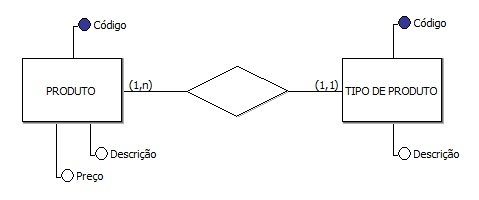
\includegraphics[width=0.6\textwidth]{img/MCD.jpg}
	\fonte{\citeonline{Heuser:2009}.}
	\label{fig:DER}
\end{figure}

%#################################################################
    \subsubsection{Modelo Entidade-Relacionamento} \label{ssec:ModeloER}
%#################################################################

Na abordagem \ac{ER} o conceito principal é o de \textbf{entidade}, o qual é uma representação de um conjunto de objetos do domínio modelado. 
As entidades são simbolizadas por retângulos. 
Contudo, nesta abordagem ainda existem também outros conceitos que são essenciais e devem ser analisados. 
Para melhor compreensão da modelagem conceitual que utiliza esta abordagem, a seguir são apresentados na \autoref{fig:ERConstrutores} algumas representações gráficas dos construtores previstos no modelo \ac{ER}. 

\begin{figure} [!htb]
    \centering
    \caption{Construtores do modelo \ac{ER}.}
    \label{fig:ERConstrutores}
    

\tikzset{every picture/.style={line width=0.75pt}} %set default line width to 0.75pt        

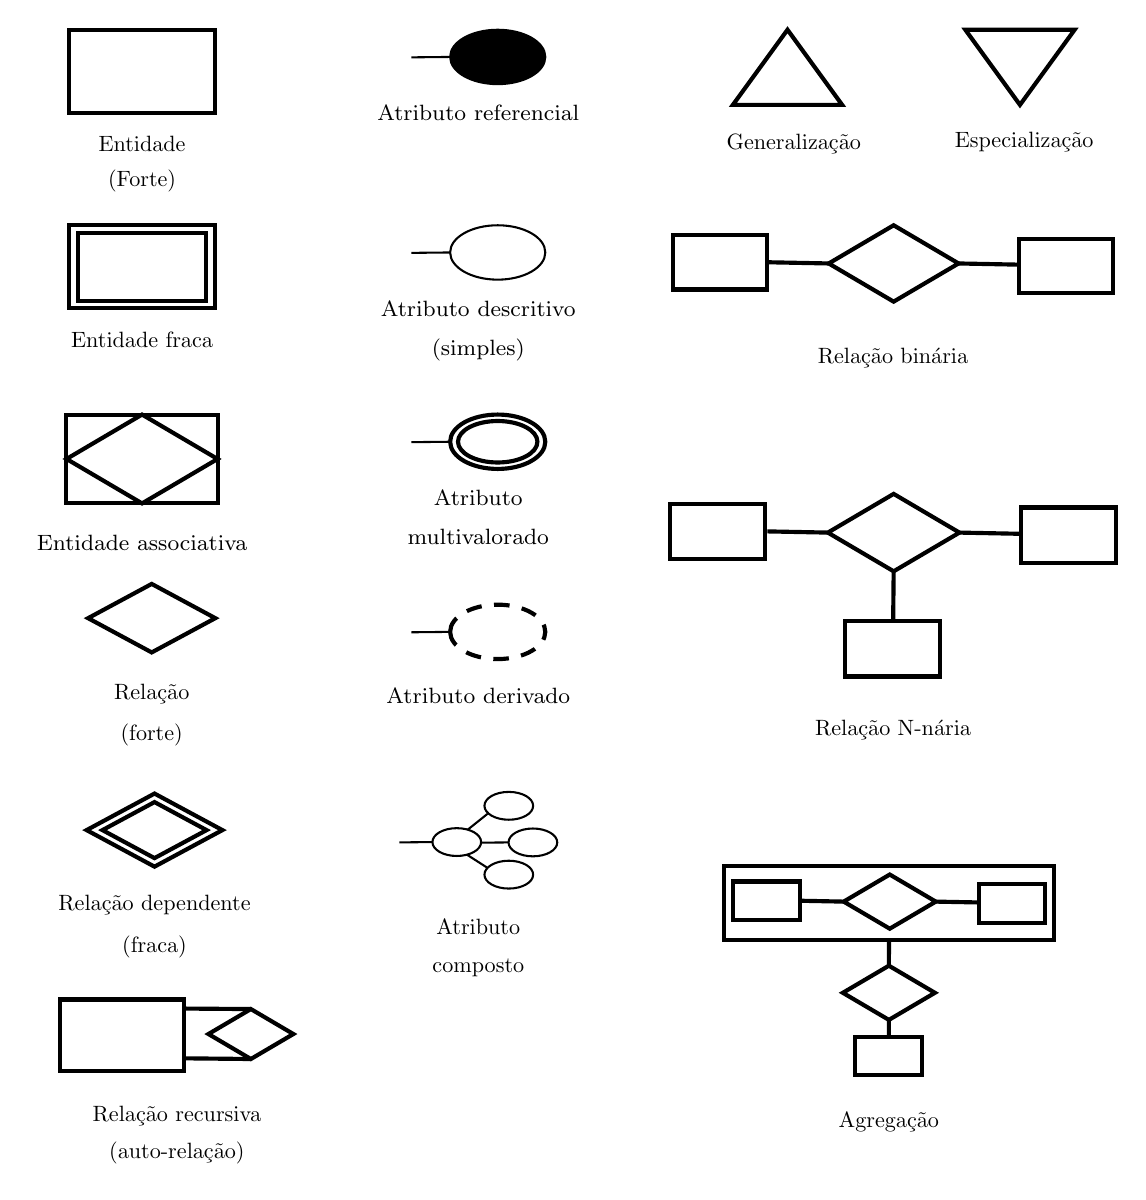
\begin{tikzpicture}[x=0.75pt,y=0.75pt,yscale=-1,xscale=1]
%uncomment if require: \path (0,597.2000122070312); %set diagram left start at 0, and has height of 597.2000122070312

%Shape: Rectangle [id:dp9409938961254447] 
\draw  [line width=1.5]  (29,15) -- (99,15) -- (99,55) -- (29,55) -- cycle ;

%Shape: Rectangle [id:dp25825363492065057] 
\draw  [line width=1.5]  (29,109.2) -- (99,109.2) -- (99,149.2) -- (29,149.2) -- cycle ;
%Shape: Rectangle [id:dp9273607878616594] 
\draw  [line width=1.5]  (33.2,112.8) -- (94.8,112.8) -- (94.8,145.6) -- (33.2,145.6) -- cycle ;

%Shape: Diamond [id:dp07590485693463012] 
\draw  [line width=1.5]  (68.65,282) -- (99.3,298.5) -- (68.65,315) -- (38,298.5) -- cycle ;

%Shape: Diamond [id:dp8393196312653484] 
\draw  [line width=1.5]  (70,383) -- (102.71,400.61) -- (70,418.22) -- (37.29,400.61) -- cycle ;
%Shape: Diamond [id:dp11016744869268091] 
\draw  [line width=1.5]  (70,387.11) -- (95.08,400.61) -- (70,414.11) -- (44.92,400.61) -- cycle ;

%Shape: Ellipse [id:dp8577075014649969] 
\draw   (212.43,122.3) .. controls (212.43,115.07) and (222.69,109.2) .. (235.35,109.2) .. controls (248.01,109.2) and (258.28,115.07) .. (258.28,122.3) .. controls (258.28,129.53) and (248.01,135.4) .. (235.35,135.4) .. controls (222.69,135.4) and (212.43,129.53) .. (212.43,122.3) -- cycle ;
%Straight Lines [id:da240419684606217] 
\draw    (193.72,122.5) -- (212.43,122.3) ;




%Shape: Ellipse [id:dp11655523259938039] 
\draw  [fill={rgb, 255:red, 0; green, 0; blue, 0 }  ,fill opacity=1 ] (212.43,28.1) .. controls (212.43,20.87) and (222.69,15) .. (235.35,15) .. controls (248.01,15) and (258.28,20.87) .. (258.28,28.1) .. controls (258.28,35.33) and (248.01,41.2) .. (235.35,41.2) .. controls (222.69,41.2) and (212.43,35.33) .. (212.43,28.1) -- cycle ;
%Straight Lines [id:da7122954732701139] 
\draw    (193.72,28.3) -- (212.43,28.1) ;




%Shape: Ellipse [id:dp23076223718363464] 
\draw  [line width=1.5]  (212.43,213.5) .. controls (212.43,206.27) and (222.69,200.4) .. (235.35,200.4) .. controls (248.01,200.4) and (258.28,206.27) .. (258.28,213.5) .. controls (258.28,220.74) and (248.01,226.6) .. (235.35,226.6) .. controls (222.69,226.6) and (212.43,220.74) .. (212.43,213.5) -- cycle ;
%Straight Lines [id:da42071644925844054] 
\draw    (193.72,213.7) -- (212.43,213.5) ;


%Shape: Ellipse [id:dp409593727665448] 
\draw  [line width=1.5]  (216.22,213.5) .. controls (216.22,207.99) and (224.78,203.51) .. (235.35,203.51) .. controls (245.92,203.51) and (254.48,207.99) .. (254.48,213.5) .. controls (254.48,219.02) and (245.92,223.49) .. (235.35,223.49) .. controls (224.78,223.49) and (216.22,219.02) .. (216.22,213.5) -- cycle ;


%Shape: Ellipse [id:dp12298573968430726] 
\draw   (203.9,406.37) .. controls (203.9,402.67) and (209.15,399.67) .. (215.63,399.67) .. controls (222.11,399.67) and (227.36,402.67) .. (227.36,406.37) .. controls (227.36,410.07) and (222.11,413.07) .. (215.63,413.07) .. controls (209.15,413.07) and (203.9,410.07) .. (203.9,406.37) -- cycle ;
%Straight Lines [id:da026255036427652145] 
\draw    (187.96,406.53) -- (203.9,406.37) ;


%Shape: Ellipse [id:dp035873659384954015] 
\draw   (228.96,388.9) .. controls (228.96,385.2) and (234.21,382.2) .. (240.69,382.2) .. controls (247.17,382.2) and (252.42,385.2) .. (252.42,388.9) .. controls (252.42,392.61) and (247.17,395.61) .. (240.69,395.61) .. controls (234.21,395.61) and (228.96,392.61) .. (228.96,388.9) -- cycle ;
%Straight Lines [id:da0884897826197295] 
\draw    (220.87,400.43) -- (230.56,392.66) ;


%Shape: Ellipse [id:dp33703819371371857] 
\draw   (240.57,406.54) .. controls (240.57,402.84) and (245.83,399.84) .. (252.31,399.84) .. controls (258.78,399.84) and (264.04,402.84) .. (264.04,406.54) .. controls (264.04,410.24) and (258.78,413.24) .. (252.31,413.24) .. controls (245.83,413.24) and (240.57,410.24) .. (240.57,406.54) -- cycle ;
%Straight Lines [id:da041465674734754376] 
\draw    (227.45,406.65) -- (240.57,406.54) ;


%Shape: Ellipse [id:dp8994114077261279] 
\draw   (228.96,422.06) .. controls (228.96,418.36) and (234.21,415.36) .. (240.69,415.36) .. controls (247.17,415.36) and (252.42,418.36) .. (252.42,422.06) .. controls (252.42,425.77) and (247.17,428.77) .. (240.69,428.77) .. controls (234.21,428.77) and (228.96,425.77) .. (228.96,422.06) -- cycle ;
%Straight Lines [id:da5145813744043246] 
\draw    (220.73,412.57) -- (230.48,418.83) ;




%Shape: Triangle [id:dp717941434970198] 
\draw  [line width=1.5]  (374.97,15) -- (401.3,51.2) -- (348.65,51.2) -- cycle ;

%Shape: Triangle [id:dp8547281306342895] 
\draw  [line width=1.5]  (486.97,51.2) -- (460.65,15) -- (513.3,15) -- cycle ;

%Shape: Ellipse [id:dp057823722753663986] 
\draw  [dash pattern={on 5.63pt off 4.5pt}][line width=1.5]  (212.43,305.1) .. controls (212.43,297.87) and (222.69,292) .. (235.35,292) .. controls (248.01,292) and (258.28,297.87) .. (258.28,305.1) .. controls (258.28,312.33) and (248.01,318.2) .. (235.35,318.2) .. controls (222.69,318.2) and (212.43,312.33) .. (212.43,305.1) -- cycle ;
%Straight Lines [id:da4937273930595423] 
\draw    (193.72,305.3) -- (212.43,305.1) ;




%Shape: Diamond [id:dp8682093873982866] 
\draw  [line width=1.5]  (426.11,109.2) -- (457.39,127.6) -- (426.11,146) -- (394.83,127.6) -- cycle ;
%Shape: Rectangle [id:dp16263593596228687] 
\draw  [line width=1.5]  (319.8,113.94) -- (365.03,113.94) -- (365.03,140.15) -- (319.8,140.15) -- cycle ;
%Shape: Rectangle [id:dp9045715408610813] 
\draw  [line width=1.5]  (486.57,115.67) -- (531.8,115.67) -- (531.8,141.89) -- (486.57,141.89) -- cycle ;
%Straight Lines [id:da894737740624673] 
\draw [line width=1.5]    (366.09,127.03) -- (394.83,127.6) ;


%Straight Lines [id:da45477038200691244] 
\draw [line width=1.5]    (457.39,127.6) -- (486.13,128.17) ;




%Shape: Diamond [id:dp8788662265812572] 
\draw  [line width=1.5]  (426.12,238.62) -- (457.82,257.27) -- (426.12,275.92) -- (394.41,257.27) -- cycle ;
%Shape: Rectangle [id:dp7607057696775741] 
\draw  [line width=1.5]  (318.35,243.42) -- (364.2,243.42) -- (364.2,270) -- (318.35,270) -- cycle ;
%Shape: Rectangle [id:dp20655084709944105] 
\draw  [line width=1.5]  (487.4,245.18) -- (533.25,245.18) -- (533.25,271.76) -- (487.4,271.76) -- cycle ;
%Straight Lines [id:da33926375234409023] 
\draw [line width=1.5]    (365.28,256.69) -- (394.41,257.27) ;


%Straight Lines [id:da8300796405989177] 
\draw [line width=1.5]    (457.82,257.27) -- (486.95,257.85) ;


%Shape: Rectangle [id:dp11640389244166749] 
\draw  [line width=1.5]  (402.47,300.05) -- (448.32,300.05) -- (448.32,326.63) -- (402.47,326.63) -- cycle ;
%Straight Lines [id:da04160890165480735] 
\draw [line width=1.5]    (425.88,299.64) -- (426.12,275.92) ;




%Shape: Diamond [id:dp09298931741553762] 
\draw  [line width=1.5]  (116.43,486.83) -- (136.89,498.86) -- (116.43,510.89) -- (95.98,498.86) -- cycle ;
%Shape: Rectangle [id:dp7562868332770196] 
\draw  [line width=1.5]  (24.66,482.2) -- (84.33,482.2) -- (84.33,516.79) -- (24.66,516.79) -- cycle ;
%Straight Lines [id:da5257649797909345] 
\draw [line width=1.5]    (84.98,510.57) -- (116.43,510.89) ;



%Straight Lines [id:da741474729938117] 
\draw [line width=1.5]    (83.76,486.58) -- (116.43,486.83) ;



%Shape: Diamond [id:dp27975998103917443] 
\draw  [line width=1.5]  (424.23,422.01) -- (446.41,435.06) -- (424.23,448.11) -- (402.04,435.06) -- cycle ;
%Shape: Rectangle [id:dp27388026856661996] 
\draw  [line width=1.5]  (348.82,425.37) -- (380.9,425.37) -- (380.9,443.97) -- (348.82,443.97) -- cycle ;
%Shape: Rectangle [id:dp8682931511633045] 
\draw  [line width=1.5]  (467.12,426.6) -- (499.19,426.6) -- (499.19,445.2) -- (467.12,445.2) -- cycle ;
%Straight Lines [id:da8247964733470876] 
\draw [line width=1.5]    (381.66,434.65) -- (402.04,435.06) ;


%Straight Lines [id:da507174915044009] 
\draw [line width=1.5]    (446.41,435.06) -- (466.8,435.46) ;


%Shape: Diamond [id:dp489563487309699] 
\draw  [line width=1.5]  (423.82,465.94) -- (446,478.99) -- (423.82,492.04) -- (401.63,478.99) -- cycle ;
%Straight Lines [id:da8803188939906841] 
\draw [line width=1.5]    (423.85,453.98) -- (423.82,465.94) ;


%Shape: Rectangle [id:dp2462964817052231] 
\draw  [line width=1.5]  (407.53,500.09) -- (439.61,500.09) -- (439.61,518.68) -- (407.53,518.68) -- cycle ;
%Straight Lines [id:da17335151983105646] 
\draw [line width=1.5]    (423.82,492.04) -- (423.83,500.08) ;


%Shape: Rectangle [id:dp019446741600327666] 
\draw  [line width=1.5]  (344.3,417.82) -- (503.3,417.82) -- (503.3,453.62) -- (344.3,453.62) -- cycle ;


%Shape: Rectangle [id:dp7508437049659447] 
\draw  [line width=1.5]  (27.54,200.66) -- (100.46,200.66) -- (100.46,242.94) -- (27.54,242.94) -- cycle ;
%Shape: Diamond [id:dp4714864707556645] 
\draw  [line width=1.5]  (64,200.4) -- (100.38,221.8) -- (64,243.2) -- (27.62,221.8) -- cycle ;



% Text Node
\draw (64,70) node [scale=0.8] [align=left] {Entidade};
% Text Node
\draw (64,88) node [scale=0.8] [align=left] {(Forte)};
% Text Node
\draw (64,164.2) node [scale=0.8] [align=left] {Entidade fraca};
% Text Node
\draw (226,55.1) node  [align=left] {{\footnotesize Atributo referencial}};
% Text Node
\draw (226,447) node [scale=0.8] [align=left] {Atributo};
% Text Node
\draw (226,467) node [scale=0.8] [align=left] {composto};
% Text Node
\draw (226,149.3) node  [align=left] {{\footnotesize Atributo descritivo}};
% Text Node
\draw (226,169.3) node  [align=left] {{\footnotesize (simples)}};
% Text Node
\draw (68.65,334.8) node [scale=0.8] [align=left] {Relação};
% Text Node
\draw (68.65,354.8) node [scale=0.8] [align=left] {(forte)};
% Text Node
\draw (70,436.8) node [scale=0.8] [align=left] {Relação dependente};
% Text Node
\draw (70,456.8) node [scale=0.8] [align=left] {(fraca)};
% Text Node
\draw (226,240.5) node  [align=left] {{\footnotesize Atributo}};
% Text Node
\draw (226,259.5) node  [align=left] {{\footnotesize multivalorado}};
% Text Node
\draw (489,69) node [scale=0.8] [align=left] {Especialização};
% Text Node
\draw (226,336.1) node  [align=left] {{\footnotesize Atributo derivado}};
% Text Node
\draw (378,70) node [scale=0.8] [align=left] {Generalização};
% Text Node
\draw (425.8,352.42) node [scale=0.8] [align=left] {Relação N-nária};
% Text Node
\draw (425.8,173.22) node [scale=0.8] [align=left] {Relação binária};
% Text Node
\draw (423.8,541.2) node [scale=0.8] [align=left] {Agregação};
% Text Node
\draw (80.78,538.2) node [scale=0.8] [align=left] {Relação recursiva};
% Text Node
\draw (80.78,556.2) node [scale=0.8] [align=left] {(auto-relação)};
% Text Node
\draw (64,262.2) node  [align=left] {{\footnotesize Entidade associativa}};


\end{tikzpicture}

    \fonte{O autor.}
\end{figure}

Uma \textbf{Entidade Forte} e uma entidade que para existir não depende da existência de outra(s) entidades(s). 
De forma inversa, uma \textbf{Entidade Fraca} é uma entidade que possui sua existência ou identificação dependente de outra(s) entidade(s). 
A representação de \textbf{Entidade Associativa} serve para dar mais sentido semântico ao modelo, e pode ser usada para simbolizar relações muitos para muitos, contendo referências a colunas de tabelas do mesmo ou de outros \acp{BD}. 

Os \textbf{atributos} podem ser \textbf{referenciais}, ou seja, que identificam a entidade, e \textbf{descritivos} que a descrevem. 
A maioria dos atributos tendem a ser descritivos e também são chamados de simples ou monovalorados. 
Contudo, existem outros tipos destes atributos como os \textbf{multivalorados}, que podem assumir diversos valores, os \textbf{derivados}, que são inferidos a partir de outros atributos, e os \textbf{compostos}, que podem ser divididos em várias partes com significados independentes.

No que diz respeito aos \textbf{relacionamentos} possíveis entre entidades pode-se citar os \textbf{binários}, aqueles que envolvem duas (2) entidades, e os \textbf{n-ários} que correspondem a ligação de três (3) ou mais entidades. 
É comum que as relações compostas especificamente por três entidades sejam chamadas de relações \textbf{ternárias}. 
Além destes tipos ainda é possível haver relações recursivas de uma entidade com ela mesma, também chamado de \textbf{auto-relacionamento}.

A abordagem \ac{ER} ainda suporta conceitos de \textbf{generalização/especialização}, que definem um grupo hierárquico de entidades que compartilham atributos em comum, e \textbf{agregação} onde a condição de existência é que o relacionamento principal necessita ser necessariamente de muitos para muitos.

Os \textbf{relacionamentos} representam a associação entre os objetos e são sinalizados por losangos. 
A \textbf{cardinalidade} de relacionamentos registra o número de ocorrências com que as entidades podem se associar. 
Existem duas cardinalidades que devem ser atribuídas: a mínima e a máxima. Os \textbf{atributos} são características representadas por pequenos círculos conectados as entidades. 
Na esquerda da \autoref{fig:DER2} é ilustrado um exemplo de \ac{DER} simples e, na direita, uma representação hipotética do conjunto de ocorrências que podem acontecer entre suas entidades. 

\begin{figure}[htb]
	\centering
	\caption{Relacionamentos e cardinalidades.}
		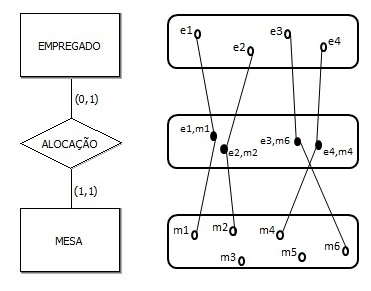
\includegraphics[width=0.5\textwidth]{img/RelCard.jpg}
	\fonte{\citeonline{Heuser:2009}.}
	\label{fig:DER2}
\end{figure}

    
%#################################################################
\subsubsection{Notações de Modelagem ER} \label{sssec:ModeloER}
%#################################################################

A abordagem \ac{ER} teve uma notação estabelecida no trabalho original de Chen, porém muitas outras notações foram propostas com o passar do tempo.
Todas essas convenções de diagramação possíveis objetivam o mesmo propósito de modelar \acp{BD}, e eventualmente podem ser utilizadas para diagramar até mesmo modelos em nível lógico como o caso da notação \textit{Crow's Foot}, conhecida pelo seu alto nível de aceitação pela indústria. 
A \autoref{fig:NotacoesER} ilustra como uma relação binária simples com cardinalidade \textit{um para muitos} pode ser representada em quatro (4) diferentes notações.

\begin{figure} [!htb]
    \centering
    \caption{Exemplos de notações para modelagem ER.}
    \label{fig:NotacoesER}
    

\tikzset{every picture/.style={line width=0.75pt}} %set default line width to 0.75pt        

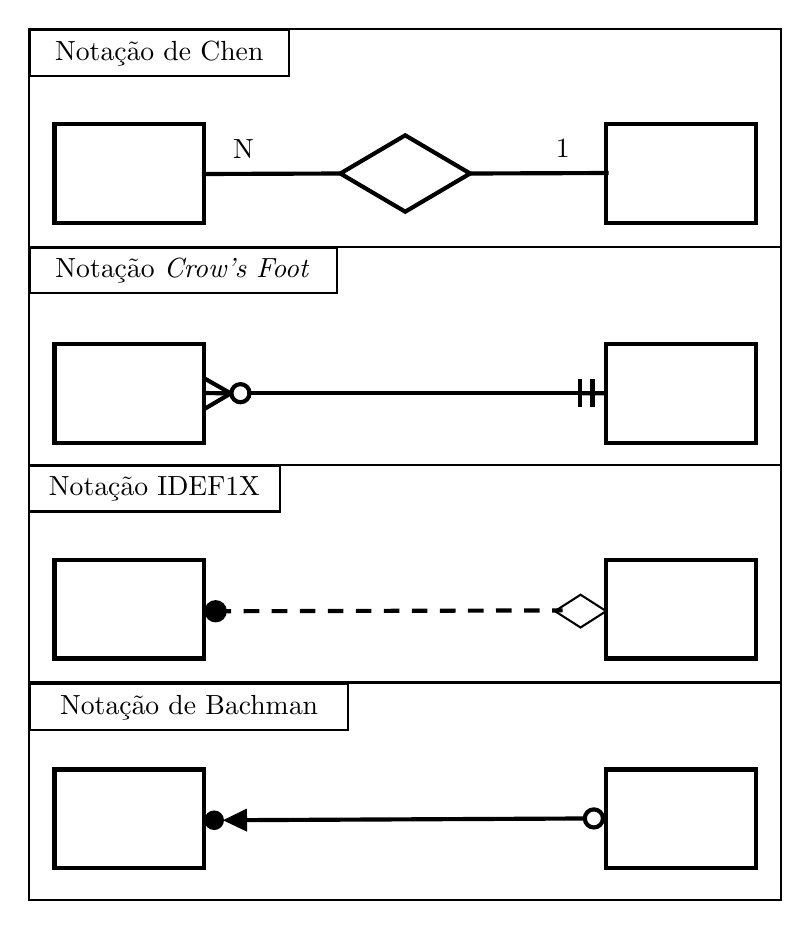
\begin{tikzpicture}[x=0.75pt,y=0.75pt,yscale=-1,xscale=1]
%uncomment if require: \path (0,525.1999969482422); %set diagram left start at 0, and has height of 525.1999969482422

%Shape: Diamond [id:dp5322960225109352] 
\draw  [line width=1.5]  (237.4,69.56) -- (268.68,87.96) -- (237.4,106.36) -- (206.13,87.96) -- cycle ;
%Shape: Rectangle [id:dp3461472448170224] 
\draw  [line width=1.5]  (68.4,64.28) -- (140.51,64.28) -- (140.51,111.63) -- (68.4,111.63) -- cycle ;
%Shape: Rectangle [id:dp4599906974909618] 
\draw  [line width=1.5]  (334.29,64.28) -- (406.4,64.28) -- (406.4,111.63) -- (334.29,111.63) -- cycle ;
%Straight Lines [id:da7414062696338117] 
\draw [line width=1.5]    (139.4,88.2) -- (206.13,87.96) ;


%Straight Lines [id:da23026930680447055] 
\draw [line width=1.5]    (268.68,87.96) -- (335.4,87.72) ;


%Shape: Rectangle [id:dp8341037786755543] 
\draw  [line width=1.5]  (68.4,274.28) -- (140.51,274.28) -- (140.51,321.63) -- (68.4,321.63) -- cycle ;
%Shape: Rectangle [id:dp31798113588606736] 
\draw  [line width=1.5]  (334.29,274.28) -- (406.4,274.28) -- (406.4,321.63) -- (334.29,321.63) -- cycle ;
%Straight Lines [id:da598335399198086] 
\draw [line width=1.5]  [dash pattern={on 5.63pt off 4.5pt}]  (146.07,298.86) -- (313.2,298.46) ;

\draw [shift={(146.07,298.86)}, rotate = 359.86] [color={rgb, 255:red, 0; green, 0; blue, 0 }  ][fill={rgb, 255:red, 0; green, 0; blue, 0 }  ][line width=1.5]      (0, 0) circle [x radius= 4.36, y radius= 4.36]   ;
%Shape: Diamond [id:dp6276925099003055] 
\draw   (321.88,290.9) -- (334.22,298.8) -- (321.88,306.7) -- (309.53,298.8) -- cycle ;
%Shape: Rectangle [id:dp5987534833309474] 
\draw  [line width=1.5]  (68.4,375.13) -- (140.51,375.13) -- (140.51,422.48) -- (68.4,422.48) -- cycle ;
%Shape: Rectangle [id:dp923966100487589] 
\draw  [line width=1.5]  (334.29,375.13) -- (406.4,375.13) -- (406.4,422.48) -- (334.29,422.48) -- cycle ;
%Straight Lines [id:da9071541568075199] 
\draw [line width=1.5]    (152.57,399.54) -- (324.93,398.7) ;
\draw [shift={(328.29,398.68)}, rotate = 359.72] [color={rgb, 255:red, 0; green, 0; blue, 0 }  ][line width=1.5]      (0, 0) circle [x radius= 4.36, y radius= 4.36]   ;
\draw [shift={(149.57,399.55)}, rotate = 359.72] [fill={rgb, 255:red, 0; green, 0; blue, 0 }  ][line width=1.5]  [draw opacity=0] (11.61,-5.58) -- (0,0) -- (11.61,5.58) -- cycle    ;
%Shape: Circle [id:dp892362699268519] 
\draw  [fill={rgb, 255:red, 0; green, 0; blue, 0 }  ,fill opacity=1 ] (141.14,399.55) .. controls (141.14,397.22) and (143.03,395.34) .. (145.35,395.34) .. controls (147.68,395.34) and (149.57,397.22) .. (149.57,399.55) .. controls (149.57,401.88) and (147.68,403.76) .. (145.35,403.76) .. controls (143.03,403.76) and (141.14,401.88) .. (141.14,399.55) -- cycle ;
%Shape: Rectangle [id:dp4762144955627674] 
\draw  [line width=1.5]  (68.4,170.28) -- (140.51,170.28) -- (140.51,217.63) -- (68.4,217.63) -- cycle ;
%Shape: Rectangle [id:dp13462140003846312] 
\draw  [line width=1.5]  (334.29,170.28) -- (406.4,170.28) -- (406.4,217.63) -- (334.29,217.63) -- cycle ;
%Straight Lines [id:da4675675836280293] 
\draw [line width=1.5]    (161.38,193.8) -- (321.62,193.8) ;
\draw [shift={(321.62,193.8)}, rotate = 180] [color={rgb, 255:red, 0; green, 0; blue, 0 }  ][line width=1.5]    (0,6.71) -- (0,-6.71)(-6.03,6.71) -- (-6.03,-6.71)   ;
\draw [shift={(158.02,193.8)}, rotate = 0] [color={rgb, 255:red, 0; green, 0; blue, 0 }  ][line width=1.5]      (0, 0) circle [x radius= 4.36, y radius= 4.36]   ;
%Straight Lines [id:da891422235378027] 
\draw [line width=1.5]    (153.37,193.9) -- (140.68,193.72) ;


%Straight Lines [id:da6698767212146683] 
\draw [line width=1.5]    (153.37,193.9) -- (141.03,186.9) ;


%Straight Lines [id:da699977038647627] 
\draw [line width=1.5]    (153.37,193.9) -- (140.37,201.57) ;


%Straight Lines [id:da3688505022442643] 
\draw [line width=1.5]    (321.62,193.8) -- (334.2,193.87) ;


%Shape: Rectangle [id:dp6749930493862317] 
\draw   (56,18.2) -- (418.3,18.2) -- (418.3,123.2) -- (56,123.2) -- cycle ;
%Shape: Rectangle [id:dp8540602211016675] 
\draw   (56,123.2) -- (418.3,123.2) -- (418.3,228.2) -- (56,228.2) -- cycle ;
%Shape: Rectangle [id:dp5100324952449573] 
\draw   (56,228.2) -- (418.3,228.2) -- (418.3,333.2) -- (56,333.2) -- cycle ;
%Shape: Rectangle [id:dp922444451928095] 
\draw   (56,333.2) -- (418.3,333.2) -- (418.3,438.2) -- (56,438.2) -- cycle ;

% Text Node
\draw (159.5,76) node  [align=left] {N};
% Text Node
\draw (313.3,76) node  [align=left] {1};
% Text Node
\draw    (56.4,19) -- (181.4,19) -- (181.4,41) -- (56.4,41) -- cycle  ;
\draw (118.9,30) node  [align=left] {Notação de Chen};
% Text Node
\draw    (56.07,228.82) -- (177.07,228.82) -- (177.07,250.82) -- (56.07,250.82) -- cycle  ;
\draw (116.57,239.82) node  [align=left] {Notação IDEF1X};
% Text Node
\draw    (56.73,334.01) -- (209.73,334.01) -- (209.73,356.01) -- (56.73,356.01) -- cycle  ;
\draw (133.23,345.01) node  [align=left] {Notação de Bachman};
% Text Node
\draw    (56.4,123.67) -- (204.4,123.67) -- (204.4,145.67) -- (56.4,145.67) -- cycle  ;
\draw (130.4,134.67) node  [align=left] {Notação \textit{Crow's Foot}};


\end{tikzpicture}

    \fonte{O autor.}
\end{figure}

%#################################################################
    \subsection{Modelo Lógico de Dados} \label{ssec:ModelLogico}
%#################################################################

Um \ac{MLD} é definido como um modelo que possui a representação dos objetos, relacionamentos e características de acordo com regras de implementação. 
Isso significa que esse modelo tem um nível de abstração do ponto de vista do usuário de um \ac{SGBD}. 
Ainda assim, o modelo lógico é independente do tipo de \ac{SGBD} em que é implementado. 
Na \autoref{fig:MLD} é apresentado um \ac{MLD} gráfico baseado no modelo da \autoref{fig:DER}.

\begin{figure}[htb]
	\centering
	\caption{Exemplo de MLD para BD relacional.}
		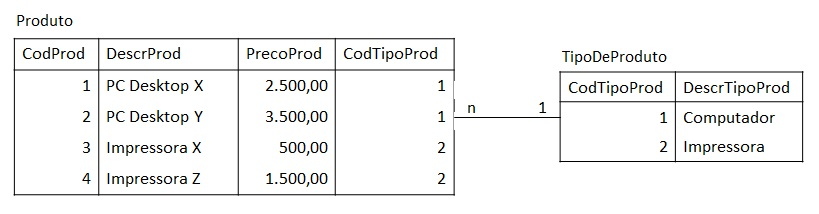
\includegraphics[width=0.8\textwidth]{img/MLD.jpg}
	\fonte{\citeonline{Heuser:2009}.}
	\label{fig:MLD}
\end{figure}

Esse tipo de modelo deve necessariamente respeitar conceitos tais como chaves de acesso, controle de chaves duplicadas, normalização, integridade referencial, controle de redundância de dados, entre outros. 
Este modelo é intrinsecamente relacionado a fase de projeto \cite{Cougo:2013}. 
É importante salientar que essa é uma forma direcionada a um aspecto gráfico, porém existem meios alternativos de se representar estruturalmente o mesmo modelo de forma textual \cite{Martelli:2018}. 
Isso é mostrado na \autoref{fig:LogicoTextual} que apresenta a definição da mesma estrutura descrita na \autoref{fig:MLD}.

\begin{figure}[!htb]
    \caption{Estrutura de um modelo lógico descrita de forma textual.}
    \label{fig:LogicoTextual}
    \centering
    \fbox{
        \parbox{13cm}{
        TipoDeProduto (\underline{CodTipoProd}, DescrTipoProd)\\
        Produto (\underline{CodProd}, DescrProd, PrecoProd, CodTipoProd)\\
        CodTipoProd referencia TipoDeProduto
        }}    
    \fonte{\citeonline{Heuser:2009}.}
\end{figure}

A obtenção de um \ac{MLD} se dá mediante a aplicação de regras de derivação sobre um \ac{MCD} já construído. 
Entretanto, não é raro que desenvolvedores e analistas experientes comecem diretamente pelo processo de modelagem lógica, ignorando a modelagem conceitual. 
Isso ocorre pois esse modelo não se preocupa somente com a representação dos objetos observados no domínio analisado, mas também com outros elementos como chaves, métodos de acesso, formatos de campo, etc. 
Isso implica, em uma última observação, que do ponto de vista formal da definição da abordagem \ac{ER}, esse modelo não se enquadra fielmente como um modelo \ac{ER} \cite{West:2011}.

%#################################################################
    \subsection{Modelo Físico de Dados} \label{ssec:ModelFisico}
%#################################################################

Um \ac{MFD} caracteriza-se como um modelo em que a representação dos objetos de \ac{BD} já estão em um nível físico de implementação das ocorrências, ou instâncias, das entidades de relacionamentos. 
Cada \ac{SGBD} pode definir diferentes modos de implementação física das características e recursos indispensáveis para o armazenamento e manipulação das estruturas de dados \cite{Cougo:2013}.

Em geral os modelos físicos apresentam dois aspectos bem representados. 
Primeiramente, existem as ocorrências ou instâncias, seus relacionamentos e a disposição básica dos elementos. 
O outro aspecto diz respeito a alocação nos diversos níveis de agrupamentos possíveis, como as tabelas, linhas (registros), colunas (campos) e blocos \cite{West:2011}.
Em suma, é a materialização dos objetos de \ac{BD} em um esquema interno de um dado \ac{SGBD} a partir da execução de uma sequência lógica de instruções em \ac{SQL}.

%#################################################################
\section{Linguagem SQL} \label{sec:LinguagemSQL}
%#################################################################

Para a manipulação dos dados a linguagem \ac{SQL} é o  padrão utilizado por sistemas de \acp{BD} relacionais disponíveis no mercado. 
A \ac{SQL} teve sua gênese originalmente nos laboratórios da IBM Research, na década de 1970, com o nome inicial de SEQUEL \cite{Chamberlin:1974}.
A \ac{SQL} é uma linguagem com a versão estável mais recente lançada em 2016 e denominada \texttt{SQL:2016}, possuindo um total de mais de 2000 páginas de especificação\footnote{https://iso.org/standard/63555.html}\footnote{https://standards.iso.org/ittf/PubliclyAvailableStandards/c065143_ISO_IEC_TR_19075-5_2016.zip}\footnote{https://standards.iso.org/ittf/PubliclyAvailableStandards/c067367_ISO_IEC_TR_19075-6_2017.zip}\footnote{https://standards.iso.org/ittf/PubliclyAvailableStandards/c069776_ISO_IEC_TR_19075-7_2017.zip}. 
Entretanto, é importante salientar que ao mesmo tempo em que a maioria dos produtos do mercado trabalham com a \ac{SQL}, estas soluções também deixam de oferecer suporte a determinados aspectos ou ainda os implementa de uma forma diferente da especificação oficial. 

A \ac{SQL} é uma única linguagem, mas comumente é categorizada conforme a funcionalidade das suas instruções. 
A primeira categoria é chamada Linguagem de Definição de Dados, do inglês \ac{DDL}. 
Entre os comandos dessa categoria estão o \texttt{CREATE}, \texttt{ALTER}, \texttt{DROP} e \texttt{TRUNCATE}. 
A segunda categoria é nomeada de Linguagem de Definição de Dados, do inglês \ac{DML}. 
Entre os comandos categorizados como \ac{DML} estão o \texttt{INSERT}, \texttt{UPDATE} e \texttt{DELETE}. 
A terceira categoria é chamada de Linguagem de Consulta de Dados, do inglês \ac{DQL}, a qual possui apenas o comando \texttt{SELECT}. 
A quarta categoria é denominada Linguagem de Transação de Dados, do inglês \ac{DTL}, a qual detém comandos como \texttt{COMMIT} e \texttt{ROLLBACK}.

A \ac{SQL} ainda utiliza uma série de cláusulas (\textit{e.g.} \texttt{FROM}, \texttt{WHERE}, \texttt{GROUP BY}, \texttt{ORDER BY}, \texttt{HAVING}, \texttt{DISTINCT}, \texttt{UNION}), operadores lógicos (\textit{e.g.} \texttt{AND}, \texttt{OR}, \texttt{NOT}), operadores relacionais (\textit{e.g.} \texttt{<}, \texttt{>}, \texttt{<=}, \texttt{>=}, \texttt{=}, \texttt{<>}) e funções de agregação (\textit{e.g.} \texttt{AVG}, \texttt{SUM}, \texttt{COUNT}, \texttt{MAX}, \texttt{MIN}). 
A aplicação destes termos e palavras reservadas, associado a características inspiradas na álgebra relacional, fundamenta a base da \ac{SQL} utilizada pelos \acp{SGBD}.

%#################################################################
    \subsection{Bancos de Dados Relacionais} \label{ssec:SGBDRelacionais}
%#################################################################

Os \acp{SGBD} relacionais suportam o modelo de dados relacional. 
O modelo de dados relacional foi proposto por \citeonline{Codd:1970} e tem como premissa a modelagem orientada a tabelas. 
Um ponto importante a ser citado é o fato de praticamente todos os \acp{SGBD} relacionais do mercado utilizarem \ac{SQL} para a criação e manipulação dos dados.

\begin{figure} [!htb]
    \centering
    \caption{Modelo de dados relacional.}
    \label{fig:ModeloRelacional}
    

\tikzset{every picture/.style={line width=0.75pt}} %set default line width to 0.75pt        

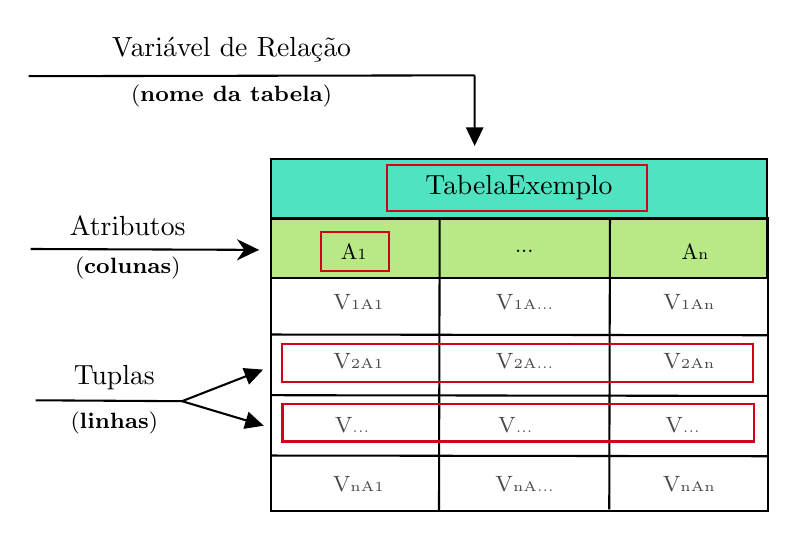
\begin{tikzpicture}[x=0.75pt,y=0.75pt,yscale=-1,xscale=1]
%uncomment if require: \path (0,456.4000015258789); %set diagram left start at 0, and has height of 456.4000015258789

%Shape: Rectangle [id:dp9895438777319416] 
\draw   (199.76,128.06) -- (439.3,128.06) -- (439.3,269.14) -- (199.76,269.14) -- cycle ;
%Straight Lines [id:da9433008870660626] 
\draw    (200.17,183.96) -- (439.3,184.31) ;


%Straight Lines [id:da2966959811071168] 
\draw    (199.96,213.19) -- (439.09,213.54) ;


%Straight Lines [id:da10336227761172356] 
\draw    (199.96,242.26) -- (439.09,242.6) ;


%Shape: Rectangle [id:dp29843450985148356] 
\draw  [fill={rgb, 255:red, 184; green, 233; blue, 134 }  ,fill opacity=1 ] (199.76,128.06) -- (439.07,128.06) -- (439.07,156.8) -- (199.76,156.8) -- cycle ;
%Straight Lines [id:da7072311505307143] 
\draw    (281.21,128) -- (280.87,268.53) ;


%Straight Lines [id:da24303755507006675] 
\draw    (363.25,127.67) -- (362.9,268.19) ;


%Straight Lines [id:da8433947995405431] 
\draw    (84.07,142.75) -- (192.19,143.17) ;
\draw [shift={(194.19,143.18)}, rotate = 180.22] [fill={rgb, 255:red, 0; green, 0; blue, 0 }  ][line width=0.75]  [draw opacity=0] (10.72,-5.15) -- (0,0) -- (10.72,5.15) -- (7.12,0) -- cycle    ;

%Shape: Rectangle [id:dp9829425897866726] 
\draw  [color={rgb, 255:red, 208; green, 2; blue, 27 }  ,draw opacity=1 ] (205.49,217.22) -- (432.44,217.22) -- (432.44,235.51) -- (205.49,235.51) -- cycle ;
%Straight Lines [id:da9003126370670107] 
\draw    (86.49,215.65) -- (157.07,216.08) ;


%Shape: Rectangle [id:dp34368494625131474] 
\draw  [color={rgb, 255:red, 208; green, 2; blue, 27 }  ,draw opacity=1 ] (205.06,188.46) -- (432,188.46) -- (432,206.75) -- (205.06,206.75) -- cycle ;
%Straight Lines [id:da28450929807989755] 
\draw    (157.07,216.08) -- (194.24,201.59) ;
\draw [shift={(196.1,200.87)}, rotate = 518.71] [fill={rgb, 255:red, 0; green, 0; blue, 0 }  ][line width=0.75]  [draw opacity=0] (8.93,-4.29) -- (0,0) -- (8.93,4.29) -- cycle    ;

%Straight Lines [id:da38844388554414944] 
\draw    (157.07,216.08) -- (194.52,227.29) ;
\draw [shift={(196.43,227.87)}, rotate = 196.67000000000002] [fill={rgb, 255:red, 0; green, 0; blue, 0 }  ][line width=0.75]  [draw opacity=0] (8.93,-4.29) -- (0,0) -- (8.93,4.29) -- cycle    ;

%Straight Lines [id:da6694551113867799] 
\draw    (83.2,59.49) -- (298.05,59.09) ;


%Shape: Rectangle [id:dp5574880153243091] 
\draw  [fill={rgb, 255:red, 80; green, 227; blue, 194 }  ,fill opacity=1 ] (199.76,99.32) -- (439.07,99.32) -- (439.07,128.06) -- (199.76,128.06) -- cycle ;
%Straight Lines [id:da8765291155015824] 
\draw    (298.05,59.09) -- (298.06,91.08) ;
\draw [shift={(298.06,93.08)}, rotate = 269.98] [fill={rgb, 255:red, 0; green, 0; blue, 0 }  ][line width=0.75]  [draw opacity=0] (8.93,-4.29) -- (0,0) -- (8.93,4.29) -- cycle    ;

%Shape: Rectangle [id:dp31459180611157866] 
\draw  [color={rgb, 255:red, 208; green, 2; blue, 27 }  ,draw opacity=1 ] (255.94,102.46) -- (381.06,102.46) -- (381.06,124.63) -- (255.94,124.63) -- cycle ;
%Shape: Rectangle [id:dp48382611043878065] 
\draw  [color={rgb, 255:red, 208; green, 2; blue, 27 }  ,draw opacity=1 ] (224.14,134.4) -- (256.9,134.4) -- (256.9,153.28) -- (224.14,153.28) -- cycle ;

% Text Node
\draw (239.74,144.01) node [scale=0.8] [align=left] {A{\scriptsize 1}};
% Text Node
\draw (321.96,144.01) node [scale=0.8] [align=left] {...};
% Text Node
\draw (404.18,144.01) node [scale=0.8] [align=left] {A{\scriptsize n}};
% Text Node
\draw (241.98,168.48) node [scale=1,color={rgb, 255:red, 74; green, 74; blue, 74 }  ,opacity=1 ] [align=left] {{\footnotesize V}{\tiny 1A1}};
% Text Node
\draw (130.91,131.43) node [scale=1] [align=left] {Atributos};
% Text Node
\draw (130.91,151.67) node [scale=1] [align=left] {{\footnotesize (\textbf{colunas})}};
% Text Node
\draw (241.98,196.46) node [scale=1,color={rgb, 255:red, 74; green, 74; blue, 74 }  ,opacity=1 ] [align=left] {{\footnotesize V}{\tiny 2A1}};
% Text Node
\draw (238.98,227.67) node [scale=1,color={rgb, 255:red, 74; green, 74; blue, 74 }  ,opacity=1 ] [align=left] {{\footnotesize V}{\tiny ...}};
% Text Node
\draw (241.98,256.17) node [scale=1,color={rgb, 255:red, 74; green, 74; blue, 74 }  ,opacity=1 ] [align=left] {{\footnotesize V}{\tiny nA1}};
% Text Node
\draw (322.14,168.48) node [scale=1,color={rgb, 255:red, 74; green, 74; blue, 74 }  ,opacity=1 ] [align=left] {{\footnotesize V}{\tiny 1A...}};
% Text Node
\draw (322.14,196.46) node [scale=1,color={rgb, 255:red, 74; green, 74; blue, 74 }  ,opacity=1 ] [align=left] {{\footnotesize V}{\tiny 2A...}};
% Text Node
\draw (317.64,227.67) node [scale=1,color={rgb, 255:red, 74; green, 74; blue, 74 }  ,opacity=1 ] [align=left] {{\footnotesize V}{\tiny ...}};
% Text Node
\draw (322.14,256.17) node [scale=1,color={rgb, 255:red, 74; green, 74; blue, 74 }  ,opacity=1 ] [align=left] {{\footnotesize V}{\tiny nA...}};
% Text Node
\draw (401.22,168.48) node [scale=1,color={rgb, 255:red, 74; green, 74; blue, 74 }  ,opacity=1 ] [align=left] {{\footnotesize V}{\tiny 1An}};
% Text Node
\draw (401.22,196.46) node [scale=1,color={rgb, 255:red, 74; green, 74; blue, 74 }  ,opacity=1 ] [align=left] {{\footnotesize V}{\tiny 2An}};
% Text Node
\draw (398.22,227.67) node [scale=1,color={rgb, 255:red, 74; green, 74; blue, 74 }  ,opacity=1 ] [align=left] {{\footnotesize V}{\tiny ...}};
% Text Node
\draw (401.22,256.17) node [scale=1,color={rgb, 255:red, 74; green, 74; blue, 74 }  ,opacity=1 ] [align=left] {{\footnotesize V}{\tiny nAn}};
% Text Node
\draw (124.43,204.59) node [scale=1] [align=left] {Tuplas};
% Text Node
\draw (124.43,226.56) node [scale=1] [align=left] {{\footnotesize (\textbf{linhas})}};
% Text Node
\draw (180.93,46.33) node [scale=1] [align=left] {Variável de Relação};
% Text Node
\draw (180.93,69.05) node [scale=1] [align=left] {{\footnotesize (\textbf{nome da tabela})}};
% Text Node
\draw (319.41,113.34) node [scale=1] [align=left] {TabelaExemplo};


\end{tikzpicture}

    \fonte{O autor.}
\end{figure}

A \autoref{fig:ModeloRelacional} mostra o esquema estrutural de um modelo relacional. Nele uma tabela, também chamada de entidade, é definida por um nome e um número fixo de atributos com seus tipos de dados indicados. 
Cada tabela deve ter um ou mais atributos identificadores, chamados de chaves, os quais auxiliam a manter a integridade referencial dos dados. 
Um registro, também chamado de ocorrência ou tupla, corresponde a uma linha na tabela e consiste nos valores de cada atributo. 
Uma relação, portanto, consiste em um conjunto de registros associados (referenciados) entre tabelas através das variáveis de relação~\cite{Ramakrishnan:2002}.

% \subsubsection{MySQL}
% O MySQL é um \ac{SGBD} relacional que foi criado por uma empresa sueca chamada MySQL AB, e atualmente é desenvolvido e mantido pela Oracle. 
% O desenvolvimento original do MySQL começou em 1994, mas a primeira versão do MySQL foi lançada apenas em maio de 1995. 
% Foi inicialmente criada para uso pessoal do \ac{SGBD} mSQL baseado na linguagem de baixo nível. 
% O MySQL é usado por muitos aplicativos da \textit{Web} orientados a \ac{BD} como o Drupal, o Joomla, o phpBB e o WordPress.
    
% Entre suas funcionalidades mais relevantes estão o suporte multiplataforma, suporte SSL, \textit{stored procedures}, \textit{triggers}, \textit{views} atualizáveis, \textit{subselects}, entre outras. 
% Atualmente, o MySQL está na versão 8.0, funciona sobre plataformas Windows, Linux, Solaris, macOS e FreeBSD. 
% Existe a versão paga \textit{Enterprise Server} e a versão de código aberto MySQL \textit{Community Server}, gratuita e com licença GPL. 
% É considerado o 2º \ac{SGBD} mais popular~\footnote{https://db-engines.com/en/system/MySQL} entre as opções do mercado pelo portal DB-Engines. 
% Segundo a avaliação publicada em 2019 pela empresa de consultoria Gartner \textit{Group}\footnote{https://gartner.com/reviews/market/operational-dbms}, o MySQL possui uma avaliação de 4,5 de 5 pelo mercado.

% \subsubsection{Microsoft SQL Server}
% O Microsoft SQL Server é um \ac{SGBD} relacional desenvolvido e mantido pela Microsoft. 
% Teve uma versão de teste foi criada em parceria com a Sybase em 1988, mas sua primeira versão para uso comercial foi lançada em abril de 1989. 
% Desde de seu lançamento este \ac{SGBD} sofreu inúmeras melhorias. 
% Atualmente possui diversas versões disponibilizadas no mercado, como a \textit{Enterprise}, a \textit{Standard}, \textit{Web}, \textit{Business Intelligence} e \textit{Workgroup}. 
    
% Também possui uma versão chamada \textit{Express}, uma edição gratuita e reduzida. 
% Essa versão inclui o mecanismo de \ac{BD} principal e, embora não haja limitações quanto ao número de \acp{BD} ou usuários com suporte, ele é limitado ao uso de um processador, 1 GB de memória e 10 GB de arquivos de \ac{BD}. 
% O Microsoft SQL Server pode funcionar sobre plataformas Linux, Microsoft Windows Server e Microsoft Windows.
% Atualmente está na versão SQL Server 2017 e é considerado o 3º \ac{SGBD} mais popular~\footnote{https://db-engines.com/en/system/Microsoft+SQL+Server} no mercado pelo portal DB-Engines. 
% Segundo a avaliação publicada pela Gartner Group, o Microsoft SQL Server possui uma avaliação de 4,4 de 5 pelo mercado em 2019.

% \subsubsection{PostgreSQL}
% O PostgreSQL é um \ac{SGBD} que incorpora o modelo relacional para seus esquemas de dados e suporta a linguagem de consulta padrão \ac{SQL}. 
% Surgiu dentro do projeto do Ingres, outro \ac{SGBD}, na universidade da Califórnia. 
% Lançado em 1996 e mantido atualmente pelo PostgreSQL Global Development Group, é considerado pelo mercado um \ac{SGBD} estável, abrangente e possuidor de boas características de desempenho. 
% É executado em praticamente qualquer plataforma Linux, macOS e Microsoft Windows. 
% O grande diferencial do PostgreSQL para ser um dos \acp{SGBD} de maior sucesso é o fato de ser gratuito e de código aberto por meio da flexível licença BSD.
    
% Entre algumas características suportadas pelo PostgreSQL estão transações, \textit{subselects}, \textit{views}, integridade referencial de chaves estrangeiras, bloqueios sofisticados, tipos definidos pelo usuário, herança, regras variadas, \textit{triggers}, funções, procedimentos armazenáveis, entre outras. 
% Atualmente está na versão 11.3 e é considerado o 4º mais popular~\footnote{https://db-engines.com/en/system/PostgreSQL} entre os \acp{SGBD} existentes pelo portal DB-Engines. 
% Segundo a avaliação publicada pela Gartner Group, o Microsoft SQL Server possui uma avaliação de 4,5 de 5 pelo mercado em 2019.

%#################################################################
\section{\textit{Model-Driven Engineering}} \label{ssec:MDE}
%#################################################################

Conceitualmente um modelo é uma representação, protótipo ou exemplo que se tem por objetivo reproduzir ou imitar de alguma forma. 
A construção de modelos são pontos centrais e importantes em diferentes áreas científicas. 
Na matemática, física e química, por exemplo, o emprego de modelos é tido como vital para a investigação teórica e prática em diferentes campos de estudo \cite{Bailer:2009}.

Em uma análise mais profunda, \citeonline{Brambilla:2017} discutem que, considerando-se a premissa de que um observador e suas observações alteram a própria realidade, é possível se concluir que tudo na percepção de um indivíduo é um modelo, já que absolutamente nada pode ser processado pela mente humana sem ser modelado. 
Em resumo, a criação de modelos é uma tarefa de abstração de domínios e conceitos do mundo real. %\cite{MS:2013}. 
Sendo assim, não é de surpreender que os modelos tenham se tornado cruciais e amplamente adotados também em áreas técnicas como mecânica, engenharia civil e, por fim, na ciência da computação, engenharia da computação e \ac{ES}.

A \ac{MDE}, também chamada de \ac{MDSE}, é uma abordagem da \ac{ES} para desenvolvimento de \textit{software} que tem essencialmente modelos como saídas principais de algum processo. 
Essa abordagem resulta em programas ou atividades de computador executados em \textit{hardware} ou \textit{software} que são gerados automaticamente a partir de modelos \cite{Sommerville:2011}. 
Conceitualmente, a \ac{MDE} fornece apoio a outros conceitos, como o \ac{MDD} e a \ac{MDA}. Na \autoref{fig:MDE_MDD_MDA} a relação entre estes conceitos é ilustrada.

\begin{figure}[!htb]
    \centering
    \caption{Relação de MDE, MDD e MDA.}
    \label{fig:MDE_MDD_MDA}
    

\tikzset{every picture/.style={line width=0.75pt}} %set default line width to 0.75pt        

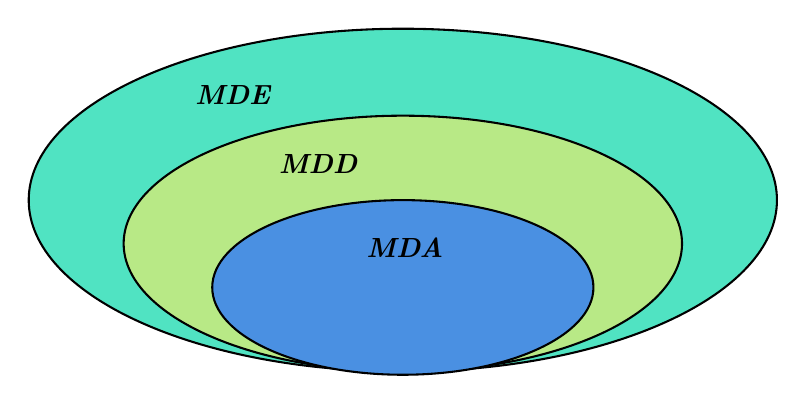
\begin{tikzpicture}[x=0.75pt,y=0.75pt,yscale=-1,xscale=1]
%uncomment if require: \path (0,300); %set diagram left start at 0, and has height of 300

%Shape: Ellipse [id:dp03875628946363818] 
\draw  [fill={rgb, 255:red, 80; green, 227; blue, 194 }  ,fill opacity=1 ] (91,113.58) .. controls (91,67.97) and (171.7,31) .. (271.25,31) .. controls (370.8,31) and (451.5,67.97) .. (451.5,113.58) .. controls (451.5,159.18) and (370.8,196.15) .. (271.25,196.15) .. controls (171.7,196.15) and (91,159.18) .. (91,113.58) -- cycle ;
%Shape: Ellipse [id:dp565416950765411] 
\draw  [fill={rgb, 255:red, 184; green, 233; blue, 134 }  ,fill opacity=1 ] (136.74,134.53) .. controls (136.74,100.49) and (196.96,72.9) .. (271.25,72.9) .. controls (345.54,72.9) and (405.76,100.49) .. (405.76,134.53) .. controls (405.76,168.56) and (345.54,196.15) .. (271.25,196.15) .. controls (196.96,196.15) and (136.74,168.56) .. (136.74,134.53) -- cycle ;
%Shape: Ellipse [id:dp0635650382067301] 
\draw  [fill={rgb, 255:red, 74; green, 144; blue, 226 }  ,fill opacity=1 ] (179.42,155.65) .. controls (179.42,132.41) and (220.53,113.58) .. (271.25,113.58) .. controls (321.97,113.58) and (363.08,132.41) .. (363.08,155.65) .. controls (363.08,178.88) and (321.97,197.72) .. (271.25,197.72) .. controls (220.53,197.72) and (179.42,178.88) .. (179.42,155.65) -- cycle ;

% Text Node
\draw (190,63) node [scale=1] [align=left] {\textit{\textbf{MDE}}};
% Text Node
\draw (231,96) node [scale=1] [align=left] {\textit{\textbf{MDD}}};
% Text Node
\draw (272.25,136.65) node [scale=1] [align=left] {\textit{\textbf{MDA}}};


\end{tikzpicture}

    \fonte{Adaptado de \citeonline{Ameller:2009}.}
\end{figure}

O \ac{MDD} é um paradigma de desenvolvimento que usa modelos como o principal artefato do processo de desenvolvimento. 
No \ac{MDD} geralmente a implementação é gerada de forma semiautomática a partir dos modelos. 
Apesar de serem vistas como a mesma coisa, o conceito da \ac{MDE} tem origem na \ac{MDA}, proposta em 2001 pelo \ac{OMG}. 
Com diferenças sutis, \citeonline{Sommerville:2011} afirma que a \ac{MDA} concentra-se nos estágios de projeto e implementação do processo de desenvolvimento de software, sendo muito similar ao \ac{MDD}, porém implementando diretrizes específicas da \ac{OMG}. 
Desta forma, conclui-se que a \ac{MDA} é um subconjunto do \ac{MDD}. 
Por outro lado, a \ac{MDE} pode abordar muitos outros tópicos do processo de \ac{ES}, entre eles a engenharia de requisitos baseada em modelos, processos de software para desenvolvimento baseado em modelos, ou ainda, testes baseados em modelos.

A \ac{MDE}, como uma metodologia, auxilia a aplicação das vantagens da modelagem nas atividades de \ac{ES}. 
Para \cite{Brambilla:2017} essa abordagem leva em consideração quatro aspectos fundamentais, listados a seguir.

\begin{enumerate}
  \item \textbf{Conceitos:} os componentes que constroem a metodologia, abrangendo desde artefatos de linguagem até atores, e assim por diante;
  \item \textbf{Notações:} A maneira como os conceitos são representados, ou seja, as linguagens usadas na metodologia;
  \item \textbf{Processos e Regras:} As atividades que levam à elaboração do produto final, as regras para sua administração e controle, e as afirmações sobre as propriedades desejadas (correção, consistência, etc) dos produtos ou do próprio processo;
  \item \textbf{Ferramentas:} Aplicações que facilitam a execução de atividades ou seu controle, abrangendo o processo de produção e apoiando o desenvolvedor no uso das notações.
\end{enumerate}

A motivação por trás da \ac{MDE} é a ideia de se aumentar o nível de abstração do processo de desenvolvimento em geral, para então assim capturar sistemas ou processos como uma coleção de modelos reutilizáveis. 
Logo, ela visa reduzir a dificuldade associada ao desenvolvimento de sistemas de software, em geral mais complexos, por meio do uso de técnicas de modelagem que suportam a separação de interesses e geração automatizada de artefatos de sistemas a partir de modelos \cite{Kleppe:2003}.

De uma forma objetiva, a abordagem \ac{MDA}, ou ainda a \ac{MDD}, é a forma de se realizar a \ac{MDE}. 
Essa abordagem define três camadas que devem ser usadas como pilares para todo o processo, listados a seguir.
A relação conceitual entre esses níveis, com o uso de mecanismos de transformação e regras de transformação, é exemplificado na \autoref{fig:MDALevels}.

\begin{enumerate}
    \item \textbf{\acp{CIM}:} descrevem objetos de negócio e as atividades independentemente de sistemas de suporte;
    \item \textbf{\acp{PIM}:} descrevem como os processos de negócio são suportados por sistemas, vistos como caixas-pretas funcionais, ou seja, desconsiderando as restrições associadas às tecnologias candidatas;
    \item \textbf{\acp{PSM}:} descrevem os componentes do sistema conforme implementados por tecnologias específicas.
\end{enumerate}

\begin{figure}[htb]
	\centering
	\caption{Níveis de abstração do MDA.}
    % 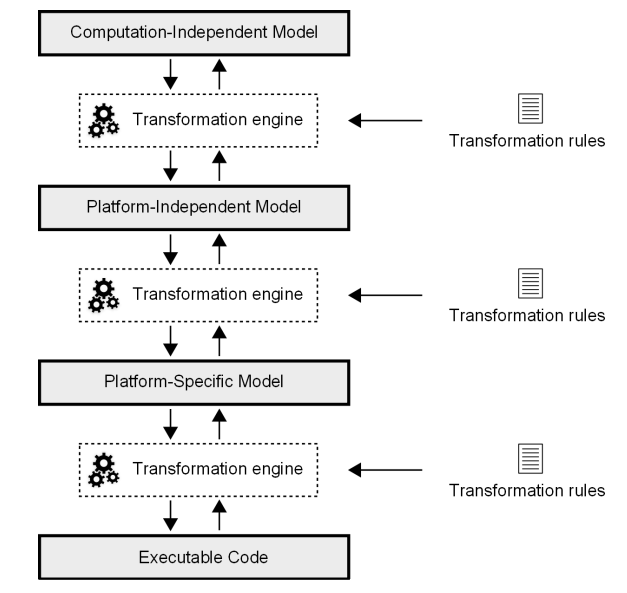
\includegraphics[width=0.57\textwidth]{img/MDA_Process.png}
    

\tikzset{every picture/.style={line width=0.75pt}} %set default line width to 0.75pt        

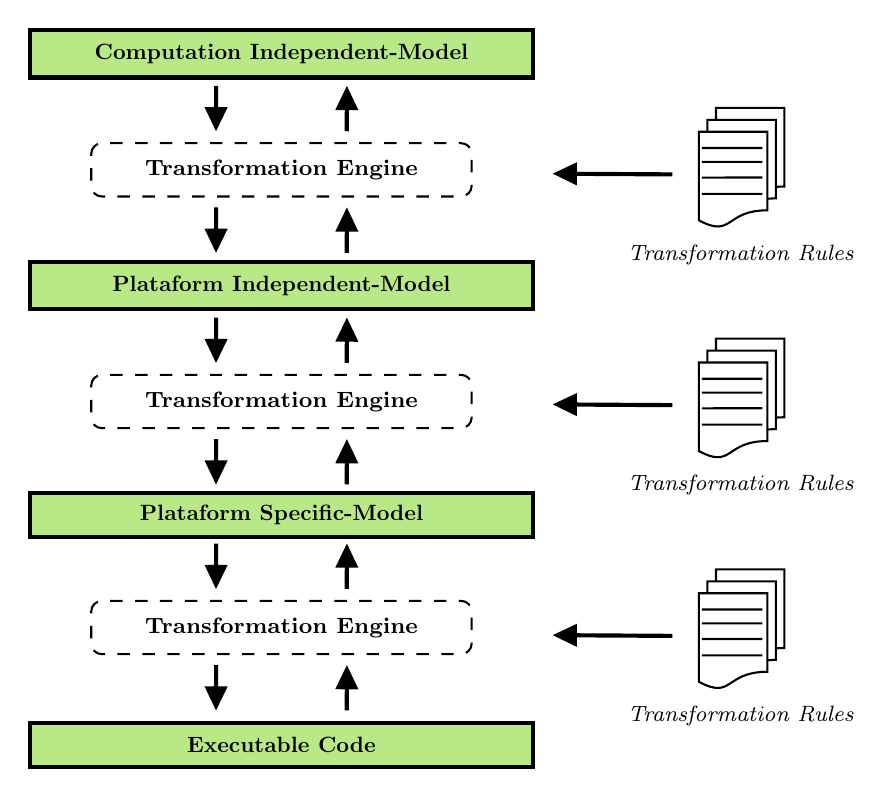
\begin{tikzpicture}[x=0.75pt,y=0.75pt,yscale=-1,xscale=1]
%uncomment if require: \path (0,442.3645935058594); %set diagram left start at 0, and has height of 442.3645935058594

%Shape: Rectangle [id:dp7655816759589134] 
\draw  [fill={rgb, 255:red, 184; green, 233; blue, 134 }  ,fill opacity=1 ][line width=1.5]  (52.59,47.21) -- (295.12,47.21) -- (295.12,70.24) -- (52.59,70.24) -- cycle ;

%Shape: Rectangle [id:dp37583246050722807] 
\draw  [fill={rgb, 255:red, 184; green, 233; blue, 134 }  ,fill opacity=1 ][line width=1.5]  (52.59,159.07) -- (295.12,159.07) -- (295.12,181.86) -- (52.59,181.86) -- cycle ;

%Shape: Rectangle [id:dp8974163182307999] 
\draw  [fill={rgb, 255:red, 184; green, 233; blue, 134 }  ,fill opacity=1 ][line width=1.5]  (52.59,270.24) -- (295.12,270.24) -- (295.12,291.66) -- (52.59,291.66) -- cycle ;

%Shape: Rectangle [id:dp7966059165934565] 
\draw  [fill={rgb, 255:red, 184; green, 233; blue, 134 }  ,fill opacity=1 ][line width=1.5]  (52.59,381.18) -- (295.12,381.18) -- (295.12,402.38) -- (52.59,402.38) -- cycle ;

%Straight Lines [id:da6759491853813937] 
\draw [line width=1.5]    (142.38,74.28) -- (142.34,93.11) ;
\draw [shift={(142.33,96.11)}, rotate = 270.14] [fill={rgb, 255:red, 0; green, 0; blue, 0 }  ][line width=1.5]  [draw opacity=0] (11.61,-5.58) -- (0,0) -- (11.61,5.58) -- cycle    ;

%Straight Lines [id:da4410578197502153] 
\draw [line width=1.5]    (205.33,96.11) -- (205.38,77.28) ;
\draw [shift={(205.39,74.28)}, rotate = 450.14] [fill={rgb, 255:red, 0; green, 0; blue, 0 }  ][line width=1.5]  [draw opacity=0] (11.61,-5.58) -- (0,0) -- (11.61,5.58) -- cycle    ;


%Rounded Rect [id:dp07358787233218322] 
\draw  [dash pattern={on 4.5pt off 4.5pt}][line width=0.75]  (82.21,106.98) .. controls (82.21,104.15) and (84.51,101.85) .. (87.35,101.85) -- (260.37,101.85) .. controls (263.2,101.85) and (265.5,104.15) .. (265.5,106.98) -- (265.5,122.4) .. controls (265.5,125.24) and (263.2,127.54) .. (260.37,127.54) -- (87.35,127.54) .. controls (84.51,127.54) and (82.21,125.24) .. (82.21,122.4) -- cycle ;

%Straight Lines [id:da6727844668924288] 
\draw [line width=1.5]    (142.38,132.84) -- (142.34,151.67) ;
\draw [shift={(142.33,154.67)}, rotate = 270.14] [fill={rgb, 255:red, 0; green, 0; blue, 0 }  ][line width=1.5]  [draw opacity=0] (11.61,-5.58) -- (0,0) -- (11.61,5.58) -- cycle    ;

%Straight Lines [id:da05695276066757793] 
\draw [line width=1.5]    (205.33,154.67) -- (205.38,135.84) ;
\draw [shift={(205.39,132.84)}, rotate = 450.14] [fill={rgb, 255:red, 0; green, 0; blue, 0 }  ][line width=1.5]  [draw opacity=0] (11.61,-5.58) -- (0,0) -- (11.61,5.58) -- cycle    ;


%Straight Lines [id:da5342535617428192] 
\draw [line width=1.5]    (142.38,185.91) -- (142.34,204.74) ;
\draw [shift={(142.33,207.74)}, rotate = 270.14] [fill={rgb, 255:red, 0; green, 0; blue, 0 }  ][line width=1.5]  [draw opacity=0] (11.61,-5.58) -- (0,0) -- (11.61,5.58) -- cycle    ;

%Straight Lines [id:da815215430339091] 
\draw [line width=1.5]    (205.33,207.74) -- (205.38,188.91) ;
\draw [shift={(205.39,185.91)}, rotate = 450.14] [fill={rgb, 255:red, 0; green, 0; blue, 0 }  ][line width=1.5]  [draw opacity=0] (11.61,-5.58) -- (0,0) -- (11.61,5.58) -- cycle    ;


%Rounded Rect [id:dp7817143384899228] 
\draw  [dash pattern={on 4.5pt off 4.5pt}][line width=0.75]  (82.21,218.61) .. controls (82.21,215.78) and (84.51,213.47) .. (87.35,213.47) -- (260.37,213.47) .. controls (263.2,213.47) and (265.5,215.78) .. (265.5,218.61) -- (265.5,234.03) .. controls (265.5,236.86) and (263.2,239.16) .. (260.37,239.16) -- (87.35,239.16) .. controls (84.51,239.16) and (82.21,236.86) .. (82.21,234.03) -- cycle ;

%Straight Lines [id:da45101461047602665] 
\draw [line width=1.5]    (142.38,244.47) -- (142.34,263.3) ;
\draw [shift={(142.33,266.3)}, rotate = 270.14] [fill={rgb, 255:red, 0; green, 0; blue, 0 }  ][line width=1.5]  [draw opacity=0] (11.61,-5.58) -- (0,0) -- (11.61,5.58) -- cycle    ;

%Straight Lines [id:da05505279480496861] 
\draw [line width=1.5]    (205.33,266.3) -- (205.38,247.47) ;
\draw [shift={(205.39,244.47)}, rotate = 450.14] [fill={rgb, 255:red, 0; green, 0; blue, 0 }  ][line width=1.5]  [draw opacity=0] (11.61,-5.58) -- (0,0) -- (11.61,5.58) -- cycle    ;


%Straight Lines [id:da8230912155193482] 
\draw [line width=1.5]    (142.38,294.79) -- (142.34,313.62) ;
\draw [shift={(142.33,316.62)}, rotate = 270.14] [fill={rgb, 255:red, 0; green, 0; blue, 0 }  ][line width=1.5]  [draw opacity=0] (11.61,-5.58) -- (0,0) -- (11.61,5.58) -- cycle    ;

%Straight Lines [id:da4013158878484284] 
\draw [line width=1.5]    (205.33,316.62) -- (205.38,297.79) ;
\draw [shift={(205.39,294.79)}, rotate = 450.14] [fill={rgb, 255:red, 0; green, 0; blue, 0 }  ][line width=1.5]  [draw opacity=0] (11.61,-5.58) -- (0,0) -- (11.61,5.58) -- cycle    ;


%Rounded Rect [id:dp7359504066475293] 
\draw  [dash pattern={on 4.5pt off 4.5pt}][line width=0.75]  (82.21,327.5) .. controls (82.21,324.66) and (84.51,322.36) .. (87.35,322.36) -- (260.37,322.36) .. controls (263.2,322.36) and (265.5,324.66) .. (265.5,327.5) -- (265.5,342.91) .. controls (265.5,345.75) and (263.2,348.05) .. (260.37,348.05) -- (87.35,348.05) .. controls (84.51,348.05) and (82.21,345.75) .. (82.21,342.91) -- cycle ;

%Straight Lines [id:da8028685074596458] 
\draw [line width=1.5]    (142.38,353.35) -- (142.34,372.18) ;
\draw [shift={(142.33,375.18)}, rotate = 270.14] [fill={rgb, 255:red, 0; green, 0; blue, 0 }  ][line width=1.5]  [draw opacity=0] (11.61,-5.58) -- (0,0) -- (11.61,5.58) -- cycle    ;

%Straight Lines [id:da3923230440168086] 
\draw [line width=1.5]    (205.33,375.18) -- (205.38,356.35) ;
\draw [shift={(205.39,353.35)}, rotate = 450.14] [fill={rgb, 255:red, 0; green, 0; blue, 0 }  ][line width=1.5]  [draw opacity=0] (11.61,-5.58) -- (0,0) -- (11.61,5.58) -- cycle    ;


%Straight Lines [id:da9965571371249939] 
\draw [line width=1.5]    (362.2,116.9) -- (307.59,116.57) ;
\draw [shift={(304.59,116.55)}, rotate = 360.35] [fill={rgb, 255:red, 0; green, 0; blue, 0 }  ][line width=1.5]  [draw opacity=0] (11.61,-5.58) -- (0,0) -- (11.61,5.58) -- cycle    ;

%Flowchart: Multidocument [id:dp4462030708787881] 
\draw  [fill={rgb, 255:red, 255; green, 255; blue, 255 }  ,fill opacity=1 ] (383.22,84.88) -- (416.2,84.88) -- (416.2,122.73) .. controls (395.59,122.73) and (399.71,136.38) .. (383.22,127.55) -- cycle ; \draw  [fill={rgb, 255:red, 255; green, 255; blue, 255 }  ,fill opacity=1 ] (379.09,90.61) -- (412.08,90.61) -- (412.08,128.46) .. controls (391.46,128.46) and (395.59,142.11) .. (379.09,133.28) -- cycle ; \draw  [fill={rgb, 255:red, 255; green, 255; blue, 255 }  ,fill opacity=1 ] (374.97,96.35) -- (407.96,96.35) -- (407.96,134.2) .. controls (387.34,134.2) and (391.46,147.85) .. (374.97,139.02) -- cycle ;
%Straight Lines [id:da3428056744320267] 
\draw    (376.37,104.19) -- (405.55,104.18) ;


%Straight Lines [id:da737270903434551] 
\draw    (376.37,110.9) -- (405.55,110.89) ;


%Straight Lines [id:da8869180718660374] 
\draw    (376.37,118.42) -- (405.55,118.4) ;


%Straight Lines [id:da4672287889638409] 
\draw    (376.37,126.31) -- (405.55,126.29) ;




%Straight Lines [id:da01844945320814495] 
\draw [line width=1.5]    (362.2,228.07) -- (307.59,227.74) ;
\draw [shift={(304.59,227.72)}, rotate = 360.35] [fill={rgb, 255:red, 0; green, 0; blue, 0 }  ][line width=1.5]  [draw opacity=0] (11.61,-5.58) -- (0,0) -- (11.61,5.58) -- cycle    ;

%Flowchart: Multidocument [id:dp3024584461272144] 
\draw  [fill={rgb, 255:red, 255; green, 255; blue, 255 }  ,fill opacity=1 ] (383.22,196.05) -- (416.2,196.05) -- (416.2,233.9) .. controls (395.59,233.9) and (399.71,247.55) .. (383.22,238.72) -- cycle ; \draw  [fill={rgb, 255:red, 255; green, 255; blue, 255 }  ,fill opacity=1 ] (379.09,201.78) -- (412.08,201.78) -- (412.08,239.64) .. controls (391.46,239.64) and (395.59,253.29) .. (379.09,244.45) -- cycle ; \draw  [fill={rgb, 255:red, 255; green, 255; blue, 255 }  ,fill opacity=1 ] (374.97,207.52) -- (407.96,207.52) -- (407.96,245.37) .. controls (387.34,245.37) and (391.46,259.02) .. (374.97,250.19) -- cycle ;
%Straight Lines [id:da8403992079487277] 
\draw    (376.37,215.36) -- (405.55,215.35) ;


%Straight Lines [id:da6998171999275149] 
\draw    (376.37,222.07) -- (405.55,222.06) ;


%Straight Lines [id:da5741349416674424] 
\draw    (376.37,229.59) -- (405.55,229.57) ;


%Straight Lines [id:da07308866987359197] 
\draw    (376.37,237.48) -- (405.55,237.46) ;




%Straight Lines [id:da3151258876682197] 
\draw [line width=1.5]    (362.2,339.24) -- (307.59,338.91) ;
\draw [shift={(304.59,338.89)}, rotate = 360.35] [fill={rgb, 255:red, 0; green, 0; blue, 0 }  ][line width=1.5]  [draw opacity=0] (11.61,-5.58) -- (0,0) -- (11.61,5.58) -- cycle    ;

%Flowchart: Multidocument [id:dp028531838068365012] 
\draw  [fill={rgb, 255:red, 255; green, 255; blue, 255 }  ,fill opacity=1 ] (383.22,307.22) -- (416.2,307.22) -- (416.2,345.07) .. controls (395.59,345.07) and (399.71,358.72) .. (383.22,349.89) -- cycle ; \draw  [fill={rgb, 255:red, 255; green, 255; blue, 255 }  ,fill opacity=1 ] (379.09,312.95) -- (412.08,312.95) -- (412.08,350.81) .. controls (391.46,350.81) and (395.59,364.46) .. (379.09,355.62) -- cycle ; \draw  [fill={rgb, 255:red, 255; green, 255; blue, 255 }  ,fill opacity=1 ] (374.97,318.69) -- (407.96,318.69) -- (407.96,356.54) .. controls (387.34,356.54) and (391.46,370.19) .. (374.97,361.36) -- cycle ;
%Straight Lines [id:da3021760556251445] 
\draw    (376.37,326.53) -- (405.55,326.52) ;


%Straight Lines [id:da14331632044731157] 
\draw    (376.37,333.24) -- (405.55,333.23) ;


%Straight Lines [id:da17482156708678565] 
\draw    (376.37,340.76) -- (405.55,340.75) ;


%Straight Lines [id:da025053397684865253] 
\draw    (376.37,348.65) -- (405.55,348.63) ;





% Text Node
\draw (173.86,58.72) node [scale=0.8] [align=left] {\textbf{Computation Independent-Model}};
% Text Node
\draw (173.86,170.46) node [scale=0.8] [align=left] {\textbf{Plataform Independent-Model}};
% Text Node
\draw (173.86,280.95) node [scale=0.8] [align=left] {\textbf{Plataform Specific-Model}};
% Text Node
\draw (173.86,391.78) node [scale=0.8] [align=left] {\textbf{Executable Code}};
% Text Node
\draw (173.86,114.69) node  [align=left] {{\footnotesize \textbf{Transformation Engine}}};
% Text Node
\draw (173.86,226.32) node  [align=left] {{\footnotesize \textbf{Transformation Engine}}};
% Text Node
\draw (173.86,335.2) node  [align=left] {{\footnotesize \textbf{Transformation Engine}}};
% Text Node
\draw (395.59,155.53) node  [align=left] {{\footnotesize \textit{Transformation Rules}}};
% Text Node
\draw (395.59,266.71) node  [align=left] {{\footnotesize \textit{Transformation Rules}}};
% Text Node
\draw (395.59,377.88) node  [align=left] {{\footnotesize \textit{Transformation Rules}}};


\end{tikzpicture}

	\fonte{Adaptado de \citeonline{Frantz:2012}.}
	\label{fig:MDALevels}
\end{figure}

Para melhor esclarecimento, os mecanismos de transformação podem ser entendidos como geradores que tem como entrada a descrição de modelos.
Esses geradores devem processar tais modelos, tendo em si implementados uma série de regras de transformação. 
Por exemplo, no contexto deste estudo um artefato de entrada seria o modelo feito utilizando a \ac{DSL} da proposta, e um mecanismo de transformação seria o gerador do modelo lógico. 
Para tanto, este gerador deve ter descritas ao todas ou parte das regras possíveis de transformação do modelo conceitual para o modelo lógico, ou seja, deve realizar o mapeamento do modelo da \ac{DSL} para um modelo relacional equivalente.
É importante salientar que estes mecanismos de transformação podem estar dispostos em vários níveis. 
Sendo assim, no contexto exemplificado é possível haver até dois (2) mecanismos de transformação: um que faz a transição do modelo conceitual para o lógico e outro que gera código \ac{SQL}.
Este último gerador ainda pode realizar esta tarefa a partir do modelo lógico previamente gerado ou mesmo diretamente do modelo conceitual. 

A separação de interesses da \ac{MDA} baseia-se, por exemplo, na exploração de diferentes \acp{DSL}, cada uma fornecendo construções baseadas em abstrações que são específicas do domínio de um sistema. 
Por conta disto, as \acp{DSL} podem desempenhar um papel de destaque na \ac{MDE} \cite{Schmidt:2006}.


%#################################################################
    \subsection{\textit{Domain-Specific Language}} \label{ssec:DSL}
%#################################################################
    
Para \citeonline{vanDeursen:2000} uma \ac{DSL} é uma linguagem de programação ou linguagem de especificação executável que oferece, por meio de notações e abstrações apropriadas, poder expressivo focado e, geralmente, restrito a um domínio de problema específico. 
Assim como outras linguagens, as \acp{DSL} devem apresentar um conjunto de sentenças bem definidas por uma sintaxe e semântica própria. 
Para \citeonline{Fowler:2010} uma \ac{DSL} é definida como uma linguagem de programação de computadores com expressividade limitada e focada em um domínio particular. 
Entre exemplos conhecidos de \acp{DSL} estão: 

\begin{itemize}
    \item \ac{SQL}, para bancos de dados;
    \item \ac{CSS}, para \textit{layout} de páginas \textit{Web};
    \item \ac{XML}, para codificação de dados;
    \item \ac{UML}, para projeto de software;
    \item \ac{SysML}, para modelagem de sistemas;
    \item \ac{VHDL}, para projeto de hardware;
    \item \LaTeX, para tipografia de documentos.
\end{itemize}
    
Segundo \citeonline{Faveri:2013}, apesar do termo \ac{DSL} poder intuitivamente remeter para um campo de estudos recente, de fato isso não é uma realidade. 
Por exemplo, a APT é uma \ac{DSL} para programação de máquinas controladas numericamente que foi desenvolvida por dois anos a partir de 1957 \cite{Ross:1978}, enquanto o formalismo de especificação de sintaxe \ac{BNF}, o mais usado para notação das linguagens de programação nos dias de hoje, remonta o final da década de 1950 \cite{Backus:1959}.
    
Em razão disso é possível encontrar na literatura muitos estudos que abordam conceitualmente \acp{DSL}, porém com diferentes terminologias.
Entre estas, pode-se citar: \textit{Languages for specialized application} \cite{Sammet:1972}; \textit{Special-purpose languages} \cite{Wexelblat:1978};  \textit{Application Languages} \cite{Martin:1982}; \textit{Task-specific programming languages} \cite{Nardi:1993}; \textit{Specialized languages} \cite{Bergin:1996}. 
    
A aplicação de \acp{DSL} permite que softwares sejam desenvolvidos de forma mais rápida e eficaz. 
A maior vantagem observada no uso de \acp{DSL} é que o conhecimento necessário para a sua aplicabilidade é abstraído para outro nível. 
Desta forma, especialistas do domínio podem entender, validar e modificar o código, adaptando o modelo as suas necessidades, tornando o impacto das mudanças mais fácil de ser compreendido. 
Também existe um aumento significativo na produtividade, confiabilidade, facilidade de uso e flexibilidade \cite{vanDeursen:2000}.

Segundo \citeonline{Mernik:2005} as \acp{DSL} podem ser classificadas sob três dimensões diferentes: \textbf{origem}, \textbf{aparência} e \textbf{implementação}. 
As dimensões de classificação de \ac{DSL} são exibidas na \autoref{fig:ClassDSL}. 
Em relação à origem de uma \ac{DSL}, as opções existentes são as \acp{DSL} \textbf{internas} e \textbf{externas}.

\begin{figure}[!htb]
    \centering
    \caption{Dimensões de uma DSL.}
    

\tikzset{every picture/.style={line width=0.75pt}} %set default line width to 0.75pt        

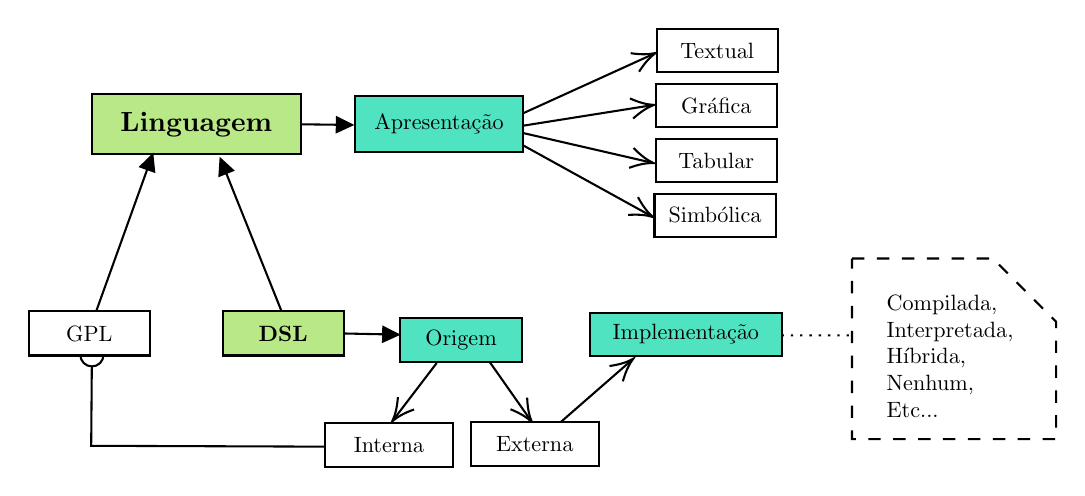
\begin{tikzpicture}[x=0.75pt,y=0.75pt,yscale=-1,xscale=1]
%uncomment if require: \path (0,408); %set diagram left start at 0, and has height of 408

%Shape: Rectangle [id:dp5982497232353539] 
\draw  [fill={rgb, 255:red, 184; green, 233; blue, 134 }  ,fill opacity=1 ] (43.96,49.84) -- (144.49,49.84) -- (144.49,78.83) -- (43.96,78.83) -- cycle ;
%Shape: Rectangle [id:dp8004700532925917] 
\draw  [fill={rgb, 255:red, 255; green, 255; blue, 255 }  ,fill opacity=1 ] (13.5,154.48) -- (71.89,154.48) -- (71.89,175.74) -- (13.5,175.74) -- cycle ;
%Shape: Rectangle [id:dp6645135942832383] 
\draw  [fill={rgb, 255:red, 184; green, 233; blue, 134 }  ,fill opacity=1 ] (106.92,154.48) -- (165.31,154.48) -- (165.31,175.74) -- (106.92,175.74) -- cycle ;
%Straight Lines [id:da940322594025554] 
\draw [fill={rgb, 255:red, 255; green, 255; blue, 255 }  ,fill opacity=1 ]   (45.99,154.48) -- (72.82,79.88) ;
\draw [shift={(73.5,78)}, rotate = 469.78] [fill={rgb, 255:red, 0; green, 0; blue, 0 }  ][line width=0.75]  [draw opacity=0] (8.93,-4.29) -- (0,0) -- (8.93,4.29) -- cycle    ;

%Straight Lines [id:da03980255509652442] 
\draw [fill={rgb, 255:red, 255; green, 255; blue, 255 }  ,fill opacity=1 ]   (135.35,154.48) -- (106.24,81.86) ;
\draw [shift={(105.5,80)}, rotate = 428.15999999999997] [fill={rgb, 255:red, 0; green, 0; blue, 0 }  ][line width=0.75]  [draw opacity=0] (8.93,-4.29) -- (0,0) -- (8.93,4.29) -- cycle    ;

%Shape: Rectangle [id:dp10111042590582864] 
\draw  [fill={rgb, 255:red, 80; green, 227; blue, 194 }  ,fill opacity=1 ] (192.6,157.7) -- (250.99,157.7) -- (250.99,178.64) -- (192.6,178.64) -- cycle ;
%Straight Lines [id:da05450643799113308] 
\draw [line width=0.75]    (165,165.11) -- (190.7,165.65) ;
\draw [shift={(192.7,165.69)}, rotate = 181.2] [fill={rgb, 255:red, 0; green, 0; blue, 0 }  ][line width=0.75]  [draw opacity=0] (8.93,-4.29) -- (0,0) -- (8.93,4.29) -- cycle    ;

%Shape: Rectangle [id:dp7588912578537257] 
\draw  [fill={rgb, 255:red, 80; green, 227; blue, 194 }  ,fill opacity=1 ] (170.72,50.8) -- (251.62,50.8) -- (251.62,77.86) -- (170.72,77.86) -- cycle ;
%Straight Lines [id:da14516072645219635] 
\draw    (168.39,64.63) -- (144.49,64.33) ;

\draw [shift={(170.38,64.65)}, rotate = 180.71] [fill={rgb, 255:red, 0; green, 0; blue, 0 }  ][line width=0.75]  [draw opacity=0] (8.93,-4.29) -- (0,0) -- (8.93,4.29) -- cycle    ;
%Straight Lines [id:da9230572726153299] 
\draw    (189.85,205.85) -- (210.08,179.33) ;

\draw [shift={(188.64,207.44)}, rotate = 307.34] [color={rgb, 255:red, 0; green, 0; blue, 0 }  ][line width=0.75]    (10.93,-4.9) .. controls (6.95,-2.3) and (3.31,-0.67) .. (0,0) .. controls (3.31,0.67) and (6.95,2.3) .. (10.93,4.9)   ;
%Straight Lines [id:da8579766023100592] 
\draw    (254.77,206.13) -- (235.75,179.06) ;

\draw [shift={(255.92,207.77)}, rotate = 234.92] [color={rgb, 255:red, 0; green, 0; blue, 0 }  ][line width=0.75]    (10.93,-4.9) .. controls (6.95,-2.3) and (3.31,-0.67) .. (0,0) .. controls (3.31,0.67) and (6.95,2.3) .. (10.93,4.9)   ;
%Straight Lines [id:da5652440770199652] 
\draw    (313.68,30.83) -- (251.75,59) ;

\draw [shift={(315.5,30)}, rotate = 155.54] [color={rgb, 255:red, 0; green, 0; blue, 0 }  ][line width=0.75]    (10.93,-4.9) .. controls (6.95,-2.3) and (3.31,-0.67) .. (0,0) .. controls (3.31,0.67) and (6.95,2.3) .. (10.93,4.9)   ;
%Straight Lines [id:da8514029171064224] 
\draw    (312.77,55.31) -- (251.75,65) ;

\draw [shift={(314.75,55)}, rotate = 170.98] [color={rgb, 255:red, 0; green, 0; blue, 0 }  ][line width=0.75]    (10.93,-4.9) .. controls (6.95,-2.3) and (3.31,-0.67) .. (0,0) .. controls (3.31,0.67) and (6.95,2.3) .. (10.93,4.9)   ;
%Shape: Rectangle [id:dp17415476114279294] 
\draw  [fill={rgb, 255:red, 255; green, 255; blue, 255 }  ,fill opacity=1 ] (226.45,207.96) -- (288.15,207.96) -- (288.15,228.89) -- (226.45,228.89) -- cycle ;
%Shape: Rectangle [id:dp5862398976742373] 
\draw  [fill={rgb, 255:red, 255; green, 255; blue, 255 }  ,fill opacity=1 ] (156.18,208.34) -- (217.88,208.34) -- (217.88,229.28) -- (156.18,229.28) -- cycle ;
%Shape: Rectangle [id:dp9794697115134454] 
\draw  [fill={rgb, 255:red, 255; green, 255; blue, 255 }  ,fill opacity=1 ] (315.61,44.77) -- (373.99,44.77) -- (373.99,65.71) -- (315.61,65.71) -- cycle ;
%Shape: Rectangle [id:dp07595309219569546] 
\draw  [fill={rgb, 255:red, 255; green, 255; blue, 255 }  ,fill opacity=1 ] (316.01,18.28) -- (374.4,18.28) -- (374.4,39.21) -- (316.01,39.21) -- cycle ;
%Shape: Rectangle [id:dp9653431753711184] 
\draw  [fill={rgb, 255:red, 80; green, 227; blue, 194 }  ,fill opacity=1 ] (283.98,155.09) -- (376.25,155.09) -- (376.25,176.03) -- (283.98,176.03) -- cycle ;
%Straight Lines [id:da6861278088536416] 
\draw    (269.62,207.98) -- (303.26,178.62) ;
\draw [shift={(304.76,177.3)}, rotate = 498.88] [color={rgb, 255:red, 0; green, 0; blue, 0 }  ][line width=0.75]    (10.93,-4.9) .. controls (6.95,-2.3) and (3.31,-0.67) .. (0,0) .. controls (3.31,0.67) and (6.95,2.3) .. (10.93,4.9)   ;

%Snip Single Corner Rect [id:dp83600176031787] 
\draw  [fill={rgb, 255:red, 255; green, 255; blue, 255 }  ,fill opacity=1 ][dash pattern={on 4.5pt off 4.5pt}] (410.17,129) -- (478.05,129) -- (508.5,159.45) -- (508.5,216) -- (410.17,216) -- cycle ;
%Straight Lines [id:da3854711457144977] 
\draw    (43.9,180.98) -- (43.6,219.23) -- (156.11,219.64) ;

\draw [shift={(43.9,180.98)}, rotate = 270.45] [color={rgb, 255:red, 0; green, 0; blue, 0 }  ][line width=0.75]      (5.59,-5.59) .. controls (2.5,-5.59) and (0,-3.09) .. (0,0) .. controls (0,3.09) and (2.5,5.59) .. (5.59,5.59) ;
%Straight Lines [id:da5105912486039843] 
\draw  [dash pattern={on 0.84pt off 2.51pt}]  (376.25,166.05) -- (409.5,166) ;


%Shape: Rectangle [id:dp1357804439753172] 
\draw  [fill={rgb, 255:red, 255; green, 255; blue, 255 }  ,fill opacity=1 ] (315.01,97.71) -- (373.4,97.71) -- (373.4,118.65) -- (315.01,118.65) -- cycle ;
%Shape: Rectangle [id:dp15166217408811944] 
\draw  [fill={rgb, 255:red, 255; green, 255; blue, 255 }  ,fill opacity=1 ] (315.51,71.28) -- (373.9,71.28) -- (373.9,92.21) -- (315.51,92.21) -- cycle ;
%Straight Lines [id:da2984867724600362] 
\draw    (312.55,82.55) -- (251.62,68.52) ;

\draw [shift={(314.5,83)}, rotate = 192.97] [color={rgb, 255:red, 0; green, 0; blue, 0 }  ][line width=0.75]    (10.93,-4.9) .. controls (6.95,-2.3) and (3.31,-0.67) .. (0,0) .. controls (3.31,0.67) and (6.95,2.3) .. (10.93,4.9)   ;
%Straight Lines [id:da44578022002737083] 
\draw    (312.5,108.03) -- (251.75,74.5) ;

\draw [shift={(314.25,109)}, rotate = 208.9] [color={rgb, 255:red, 0; green, 0; blue, 0 }  ][line width=0.75]    (10.93,-4.9) .. controls (6.95,-2.3) and (3.31,-0.67) .. (0,0) .. controls (3.31,0.67) and (6.95,2.3) .. (10.93,4.9)   ;

% Text Node
\draw (94.23,64.33) node [scale=1] [align=left] {\textbf{Linguagem}};
% Text Node
\draw (42.69,165.11) node [scale=0.8] [align=left] {GPL};
% Text Node
\draw (136.11,165.11) node [scale=0.8] [align=left] {\textbf{DSL}};
% Text Node
\draw (221.79,168.17) node [scale=0.8] [align=left] {Origem};
% Text Node
\draw (257.3,218.42) node [scale=0.8] [align=left] {Externa};
% Text Node
\draw (187.03,218.81) node [scale=0.8] [align=left] {Interna};
% Text Node
\draw (344.8,55.24) node [scale=0.8] [align=left] {Gráfica};
% Text Node
\draw (345.21,28.75) node [scale=0.8] [align=left] {Textual};
% Text Node
\draw (211.17,64.33) node [scale=0.8] [align=left] {Apresentação};
% Text Node
\draw (330.11,165.56) node [scale=0.8] [align=left] {Implementação};
% Text Node
\draw (457.39,176.08) node [scale=0.8] [align=left] {Compilada, \\Interpretada,\\Híbrida, \\Nenhum, \\Etc...};
% Text Node
\draw (344.21,108.18) node [scale=0.8] [align=left] {Simbólica};
% Text Node
\draw (344.71,81.75) node [scale=0.8] [align=left] {Tabular};


\end{tikzpicture}

    \label{fig:ClassDSL}
    \fonte{Adaptado de  \citeonline{Faveri:2013}.}
\end{figure}
    
Uma \ac{DSL} \textbf{interna} é projetada a partir das regras sintáticas e semânticas da gramática de uma linguagem já existente, podendo ser essa uma linguagem de propósito geral, do inglês \ac{GPL}, ou outra \ac{DSL}. 
Sendo assim, para seu funcionamento correto uma \ac{DSL} interna acaba transferindo todas as atividades de verificação léxica, sintática, semântica e de transformação de código ao compilador da linguagem hospedeira.

Uma \ac{DSL} \textbf{externa} é uma linguagem com sintaxe distinta e que depende de uma infraestrutura própria para a análise léxica, sintática, semântica, interpretação, compilação, otimização e geração de código. 
Se comparada a uma \ac{GPL}, uma \ac{DSL} externa possui especificidades similares, porém seus recursos são restritos ao domínio de aplicação para o qual a linguagem é projetada.
    
No que diz respeito à dimensão de \textbf{aparência}, uma \ac{DSL} pode ser classificada como \textbf{textual}, \textbf{gráfica}, \textbf{tabular} e \textbf{simbólica}. 
Quando no formato textual as \acp{DSL} permitem que o domínio seja expressado com caracteres, os quais são então combinados gerando palavras, expressões, sentenças e instruções que seguem as regras gramaticais previamente estabelecidas na linguagem. 
As \acp{DSL} não textuais seguem a mesma lógica, mas utilizando-se de modelos gráficos para permitir que o usuário possa expressar conhecimento de domínio com um maior nível de compreensão e empregando para tal o uso de símbolos, tabelas, figuras e conectores. 
    
E finalmente, no que se refere a dimensão de \textbf{implementação}, as \acp{DSL} podem ser classificadas tendo em vista a perspectiva de sua execução. 
Essas classificações formam quatro grupos: 
(i) \acp{DSL} de execução bem definidas (\textit{e.g.} Excel Macro Language); 
(ii) \acp{DSL} que servem de entrada para geradores de aplicação; 
(iii) \acp{DSL} não executáveis mas úteis como entrada de geradores de aplicação; 
(iv) \acp{DSL} não projetadas para serem executadas.

É prática usual que o principal aspecto levado em consideração para a construção de uma \acp{DSL} deve ser a sua \textbf{origem}, pois cada abordagem apresenta vantagens e desvantagens específicas que são inerentes a cada tipo \cite{Fowler:2010}. 
Apesar das \acp{DSL} externas poderem ter um esforço associado a sua construção muitas vezes maior do que o de uma \ac{DSL} interna, atualmente existem ferramentas que dão grande suporte a construção de \acp{DSL}. 
Estas ferramentas são conhecidas como \acp{LW} e aplicam conceitos de programação orientada a linguagens, fornecendo um nível de abstração maior no que diz respeito as questões complexas de infraestrutura \cite{Fowler:2005}.
    
%#################################################################    
\subsection{\textit{Language Workbenches}} \label{ssec:LW}
%#################################################################

O desenvolvimento de uma \ac{DSL} não é tarefa trivial pois, como são linguagens de programação, possuem uma sintaxe que é, por consequência lógica, definida por uma gramática. 
Desta forma, se faz necessária a utilização de ferramentas que suportem a definição dos conceitos para a nova linguagem \cite{Fowler:2005}.

Os \acp{LW} são ferramentas que fornecem mecanismos de infraestrutura para a implementação de linguagens de programação, tornando assim a criação de linguagens mais acessível \cite{Wachsmuth:2014}. 
Entre os mecanismos fornecidos nesses ambientes está a formatação automática, validação com base nas restrições descritas na gramática, \textit{syntax highlighting}\footnote{Realce de código-fonte com cor, negrito, etc. Serve para indicar sua estrutura sintática.} e \textit{syntax completion}\footnote{Uma função, como em um mecanismo de busca, que fornece uma ou mais opções de palavras reservadas previstas na gramática a partir dos caracteres que um usuário já inseriu.}. 
A seguir são citados alguns dos mais conhecidos \acp{LW} da atualidade:

\begin{itemize}
    \item \textbf{Xtext:} lançado em 2006, o Xtext é um \textit{framework} de código aberto para o desenvolvimento linguagens de programação textuais, com integração com o ambiente de desenvolvimento integrado, do inglês \ac{IDE}, Eclipse. 
    Para especificar uma linguagem, o desenvolvedor descreve uma gramática no Xtext. 
    Essa gramática descreve como um modelo \textit{Ecore} deve ser derivado de uma notação textual. 
    A partir dessa definição, um gerador de código deriva um analisador ANTLR e as classes para o modelo de objetos. 
    O Xtext também tem um gerador Xtend editável, o que dá a capacidade de se gerar código para qualquer outra gramática. 
    O Xtext inclui recursos inerentes ao \ac{IDE} Eclipse como \textit{syntax highlighting}, \textit{code completion}, \textit{static analysis}, \textit{source-code navigation} e outros. 
    Atualmente está na versão 2.18.0.
    
    \item \textbf{Sirius:} lançado em 2007 em um esforço entre as empresas Thales e Obeo, atualmente o \textit{framework} Sirius é um projeto de licença aberta mantido pela Eclipse Foundation, cujo objetivo é permitir a criação de ferramentas de modelagem. 
    Com o Sirius é possível especificar \acp{DSL} visuais e gerar assim a infraestrutura de editores gráficos.
    O Sirius, assim como o Xtext, possui integração com recursos específicos do ambiente Eclipse. Atualmente está na versão 6.2.1.
    
    \item \textbf{JetBrains MPS:} o JetBrains MPS é um sistema desenvolvido pela JetBrains, empresa da República Tcheca, que usa edição projetiva. 
    Essa abordagem permite aos desenvolvedores uma melhor compreensão, o que a diferencia de outros \acp{LW}. 
    Também possui funções comuns de \acp{IDE} integrado a seu ambiente de desenvolvimento. 
    Está atualmente na versão 2019.1.1 sob a licença Apache 2.0.
    
    \item \textbf{MetaEdit+:} o MetaEdit+ é \ac{LW} proprietário desenvolvido pela companhia finlandesa MetaCase para criar e utilizar \acp{DSL}. 
    Possui duas versões nomeadamente \textit{MetaEdit+ Workbench} e \textit{MetaEdit Modeler}. 
    O \textit{Workbench} inclui ferramentas para projetar e usar/testar linguagens de modelagem enquanto o Modeler inclui ferramentas para se utilizar linguagens de modelagem. 
    Normalmente, o \textit{MetaEdit+ Workbench} é usado pelos desenvolvedores que projetam uma \ac{DSL} do domínio para um projeto. 
    Em seguida, essa linguagem de modelagem é usada para desenvolver produtos finais com o apoio do \textit{MetaEdit+ Modeler}. 
    Atualmente está na versão 5.5 SR1.
\end{itemize}

É interessante salientar que a capacidade de definir referências cruzadas fornecida por \acp{LW} é o que os torna mais atrativos para o desenvolvimento rápido de \acp{DSL}. Observando por um lado prático, essa capacidade é ainda mais notável em \acp{LW} como o Xtext, uma vez que essa plataforma proporciona abstração suficiente para a realizar a especificação de \acp{GLC} executáveis.

%#################################################################    
\section{Gramáticas Livres de Contexto} \label{ssec:GLC}
%#################################################################

Na matemática, ciência da computação e linguística, uma linguagem formal consiste em palavras cujas letras são retiradas de um alfabeto e são bem formadas de acordo com um conjunto específico de regras. 
Existem diversas abordagens computacionais que tem por objetivo proporcionar que os computadores possam compreender a \ac{LN} falada e/ou escrita por humanos. 
Compreender neste cenário significa, no mínimo, reconhecer o contexto, fazer análise sintática, semântica, léxica e morfológica. 
Esse conjunto de técnicas computacionais compõem uma área denominada \ac{PLN} \cite{Jurafsky:2009}.

Contudo, mesmo com a evolução tecnológica proporcionada pelo esforço de diversos pesquisadores, a comunicação entre homem e máquina através de \ac{LN} continua sendo um desafio. 
Ainda assim, por ser uma área vasta o \ac{PLN} engloba diversos espectros onde as linguagens podem ser classificadas conforme as regras de formação e sua expressividade. 
Neste sentido a figura do filósofo, linguista e escritor norte-americano Noan Chomsky é um expoente, uma vez que ele estabeleceu uma teoria em 1959 que descreve um conjunto de quatro (4) níveis para a classificação de qualquer linguagem. 
A teoria mostra que há quatro (4) classes de gramáticas capazes de gerar diferentes linguagens \cite{Linz:2016}.

Posteriormente o modelo proposto foi refinado por outros pesquisadores, e conta atualmente com versões de até sete (7) níveis. 
Em razão do foco deste estudo ser uma \ac{GLC}, será abordado o nível dois (2) da definição clássica de Chomsky, expressada na Figura \ref{fig:Chomsky}.

\begin{figure}[!htb]
    \centering
    \caption{Representação dos níveis da Hierarquia de Chomsky.}
    \label{fig:Chomsky}
    

\tikzset{every picture/.style={line width=0.75pt}} %set default line width to 0.75pt        

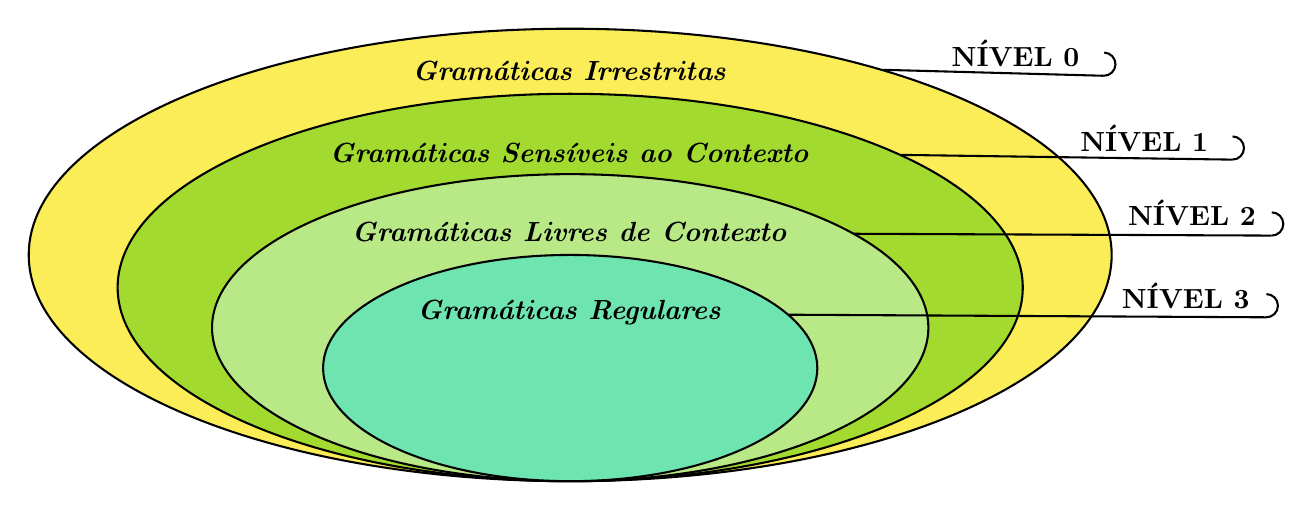
\begin{tikzpicture}[x=0.75pt,y=0.75pt,yscale=-1,xscale=1]
%uncomment if require: \path (0,478.1979217529297); %set diagram left start at 0, and has height of 478.1979217529297

%Shape: Ellipse [id:dp2589253237302658] 
\draw  [fill={rgb, 255:red, 248; green, 231; blue, 28 }  ,fill opacity=0.74 ] (8.59,137.21) .. controls (8.59,77.01) and (125.4,28.21) .. (269.48,28.21) .. controls (413.56,28.21) and (530.36,77.01) .. (530.36,137.21) .. controls (530.36,197.41) and (413.56,246.21) .. (269.48,246.21) .. controls (125.4,246.21) and (8.59,197.41) .. (8.59,137.21) -- cycle ;
%Shape: Ellipse [id:dp694350790161383] 
\draw  [fill={rgb, 255:red, 126; green, 211; blue, 33 }  ,fill opacity=0.71 ] (51.43,152.88) .. controls (51.43,101.34) and (149.05,59.56) .. (269.48,59.56) .. controls (389.91,59.56) and (487.53,101.34) .. (487.53,152.88) .. controls (487.53,204.43) and (389.91,246.21) .. (269.48,246.21) .. controls (149.05,246.21) and (51.43,204.43) .. (51.43,152.88) -- cycle ;
%Shape: Ellipse [id:dp7384199846467594] 
\draw  [fill={rgb, 255:red, 184; green, 233; blue, 134 }  ,fill opacity=1 ] (96.92,172.24) .. controls (96.92,131.39) and (174.18,98.28) .. (269.48,98.28) .. controls (364.78,98.28) and (442.04,131.39) .. (442.04,172.24) .. controls (442.04,213.09) and (364.78,246.21) .. (269.48,246.21) .. controls (174.18,246.21) and (96.92,213.09) .. (96.92,172.24) -- cycle ;
%Shape: Ellipse [id:dp08042679579621703] 
\draw  [fill={rgb, 255:red, 80; green, 227; blue, 194 }  ,fill opacity=0.7 ] (150.42,191.71) .. controls (150.42,161.61) and (203.72,137.21) .. (269.48,137.21) .. controls (335.24,137.21) and (388.54,161.61) .. (388.54,191.71) .. controls (388.54,221.81) and (335.24,246.21) .. (269.48,246.21) .. controls (203.72,246.21) and (150.42,221.81) .. (150.42,191.71) -- cycle ;
%Straight Lines [id:da6929823208677994] 
\draw    (420,48) -- (526.44,50.88) ;
\draw [shift={(526.44,50.88)}, rotate = 181.55] [color={rgb, 255:red, 0; green, 0; blue, 0 }  ][line width=0.75]      (0,0) .. controls (-3.09,0) and (-5.59,2.5) .. (-5.59,5.59) .. controls (-5.59,8.68) and (-3.09,11.18) .. (0,11.18) ;

%Straight Lines [id:da9940150469857363] 
\draw    (429,89) -- (588.44,91.28) ;
\draw [shift={(588.44,91.28)}, rotate = 180.82] [color={rgb, 255:red, 0; green, 0; blue, 0 }  ][line width=0.75]      (0,0) .. controls (-3.09,0) and (-5.59,2.5) .. (-5.59,5.59) .. controls (-5.59,8.68) and (-3.09,11.18) .. (0,11.18) ;

%Straight Lines [id:da8023852859401694] 
\draw    (406,127) -- (607.44,127.88) ;
\draw [shift={(607.44,127.88)}, rotate = 180.25] [color={rgb, 255:red, 0; green, 0; blue, 0 }  ][line width=0.75]      (0,0) .. controls (-3.09,0) and (-5.59,2.5) .. (-5.59,5.59) .. controls (-5.59,8.68) and (-3.09,11.18) .. (0,11.18) ;

%Straight Lines [id:da75358331134597] 
\draw    (375,166) -- (604.84,167.25) ;
\draw [shift={(604.84,167.25)}, rotate = 180.31] [color={rgb, 255:red, 0; green, 0; blue, 0 }  ][line width=0.75]      (0,0) .. controls (-3.09,0) and (-5.59,2.5) .. (-5.59,5.59) .. controls (-5.59,8.68) and (-3.09,11.18) .. (0,11.18) ;


% Text Node
\draw (269.48,48.76) node [scale=1] [align=left] {\textbf{\textit{Gramáticas Irrestritas}}};
% Text Node
\draw (269.48,126.28) node [scale=1] [align=left] {\textbf{\textit{Gramáticas Livres de Contexto}}};
% Text Node
\draw (269.48,88.11) node [scale=1] [align=left] {\textbf{\textit{Gramáticas Sensíveis ao Contexto}}};
% Text Node
\draw (269.48,164.97) node [scale=1] [align=left] {\textbf{\textit{Gramáticas Regulares}}};
% Text Node
\draw (484,40) node  [align=left] {\textbf{NÍVEL 0}};
% Text Node
\draw (546,81) node  [align=left] {\textbf{NÍVEL 1}};
% Text Node
\draw (569,117) node  [align=left] {\textbf{NÍVEL 2}};
% Text Node
\draw (566,157) node  [align=left] {\textbf{NÍVEL 3}};


\end{tikzpicture}

    \fonte{O autor.}
\end{figure}

Nesta hierarquia toda a classe de gramática é um subconjunto da classe do nível imediatamente acima. 
Por exemplo, toda linguagem livre de contexto também é sensível ao contexto, porém a situação inversa não é sempre verdadeira. 
As \acp{GLC} são poderosas o suficiente para descrever a sintaxe da maioria das linguagens de programação utilizadas na atualidade.

Segundo \citeonline{Linz:2016}, as gramáticas consistem de uma coleção de regras de substituição, também chamadas de produções. 
Cada regra aparece como uma linha na gramática, compreendendo um símbolo e uma cadeia separados por uma seta. 
Estas regras descrevem como as cadeias podem ser reconhecidas ou formadas. 
Uma \ac{GLC} é uma gramática formal em que cada regra de produção é da forma $V \rightarrow w$, onde $V$ é um único símbolo não-terminal(variável) e $w$ é uma cadeia de terminais e/ou variáveis, podendo ainda ser também uma cadeia vazia (palavra vazia). 
O termo "livre de contexto" expressa basicamente o fato de que um $V$ não terminal sempre pode ser substituído por $w$, independentemente do contexto em que ocorre.

Demonstrando em um exemplo simples, a linguagem $L=\{a^{n}b^{n}:n \geq 1\}$ define uma estrutura onde todas as cadeias de caracteres são não vazias, de tamanho par e tem a primeira metade preenchida por "a"s e a segunda metade sempre por "b"s. 
Algumas palavras que essa linguagem aceita são $ab$, $aabb$ e $aaabbb$.
Um exemplo de \ac{GLC} que consegue gerá-las é  ${S\to aSb~|~ab}$, contudo é importante salientar que dependendo da linguagem diferentes gramáticas podem gerá-las.

%#################################################################    
\subsection{Formalismo de Backus-Naur} \label{sssec:BNF}
%#################################################################

A primeira representação da gramática de uma linguagem de programação foi apresentada por John Backus, em 1959, para expressar a linguagem 
Algol. Esta notação seguia o mesmo padrão de \acp{GLC} estudado por linguistas como Chomsky, dando origem a notação \ac{BNF} \cite{Edelweiss:2014}.

A notação \ac{BNF} é utilizada para expressar \acp{GLC} e, em geral, é amplamente empregada para a especificação de \acp{GPL}. 
Porém é uma notação que não se restringe apenas as \acp{GPL}, sendo usada também para expressar protocolos de comunicação, formato de dados e outros tipos de linguagens como as específicas de domínio. 
Em geral não é usado em língua natural porque essa notação não é adequada para gramáticas que dependem de contexto.

Na notação \ac{BNF} é simples e muito similar ao modelo utilizado no campo da linguística para definição de \acp{GLC} pois nela: (\textbf{I}) as variáveis são palavras entre os símbolos $\langle$ e $\rangle$ ; (\textbf{II}) as palavras não delimitadas são terminais; (\textbf{III}) a regra geral de produção ${S\to \alpha}$ é representada como ${S ::= \alpha}$, ou ainda, $\langle SNT \rangle ::= \langle \alpha T~|~\alpha T~+~SNT \rangle$. 

Para compreensão, o "\texttt{$::=$}"~ indica "\textit{é definido como}", o \texttt{$|$} indica "\textit{ou}"~ e os colchetes angulares (\texttt{$\langle~\rangle$}) distinguem nomes de regras de sintaxe, chamados de símbolos não terminais (SNT), dos símbolos de terminais (\texttt{$\alpha T$}) que são escritos exatamente como devem ser representados, sendo estes últimos também conhecidos como palavras reservadas. 
Um exemplo da aplicação da notação \ac{BNF} para definir a estrutura de uma mini-linguagem de programação pode ser expressada conforme a \autoref{fig:MiniLanguage}.
\definecolor{javared}{rgb}{0.6,0,0} % for strings
\definecolor{javagreen}{rgb}{0.25,0.5,0.35} % comments
\definecolor{javapurple}{rgb}{0.5,0,0.35} % keywords
\definecolor{javadocblue}{rgb}{0.25,0.35,0.75} % javadoc
\definecolor{verde}{rgb}{0.25,0.5,0.35}
\definecolor{jpurple}{rgb}{0.5,0,0.35}
\definecolor{darkgreen}{rgb}{0.0, 0.2, 0.13}


\lstdefinelanguage{Xtext}{
  sensitive = true,
  keywords={},
  keywords=[2]{ERModel, Domain, Attribute, Entity, Relation, RelationSide, DataType, CardinalityType},
  keywords=[3]{grammar, with, generate, Terminals, enum},
  otherkeywords={*, ?, +, *=, ?=, +=, |},
  keywordstyle=\color{black}\bfseries,
  keywordstyle=[2]\color{javadocblue}\bfseries,
  keywordstyle=[3]\color{javapurple}\bfseries,% for example
%   backgroundcolor=\color{cyan!10},
%   numbers=left,
%   stepnumber=1,
  numbersep=8pt,
  showstringspaces=false,
  breaklines=true,
  frame=top,
  comment=[l]{//},
  morecomment=[s]{/*}{*/},
  commentstyle=\color{black}\ttfamily,
  stringstyle=\color{javared}\ttfamily,
  morestring=[b]',
  morestring=[b]"
  }
  
  \lstdefinelanguage{ERDSL}{
  sensitive = true,
  keywords={},
  keywords=[2]{Domain, Entities, Relationships, isIdentifier, isRelatedWith, isA, zero, one, many},
  keywords=[3]{int, money, string, datetime, file},
  otherkeywords={*, ?, +, *=, ?=, +=, |},
  keywordstyle=\color{black}\bfseries,
  keywordstyle=[2]\color{javapurple}\bfseries,
  keywordstyle=[3]\color{javadocblue}\bfseries,% for example
%   backgroundcolor=\color{cyan!10},
%   numbers=left,
%   stepnumber=1,
  captionpos=t,
  numbersep=8pt,
  showstringspaces=false,
  breaklines=true,
  frame=top,
  comment=[l]{//},
  morecomment=[s]{/*}{*/},
  commentstyle=\color{black}\ttfamily,
  stringstyle=\color{javared}\ttfamily,
  morestring=[b]',
  morestring=[b]"
  }
  
  \lstdefinelanguage{BNF}{
  sensitive = true,
  keywords={},
  keywords=[2]{},
  otherkeywords={::= , |, <, >},
  keywordstyle=\color{javapurple}\bfseries,
  keywordstyle=[2]\color{javapurple}\bfseries,
  keywordstyle=[3]\color{javadocblue}\bfseries,% for example
%   backgroundcolor=\color{cyan!10},
%   numbers=left,
%   stepnumber=1,
  captionpos=t,
  numbersep=8pt,
  showstringspaces=false,
  breaklines=true,
  frame=top,
  comment=[l]{//},
  morecomment=[s]{/*}{*/},
  commentstyle=\color{darkgreen}\ttfamily,
  stringstyle=\color{javared}\ttfamily,
  morestring=[b]',
  morestring=[b]"
  }
  
  
  
  

\begin{figure}[!htb]
    \centering
    \caption{Exemplo de mini-linguagem definida com BNF.}
    \label{fig:MiniLanguage}
    \begin{scriptsize}
    \begin{lstlisting}[language = BNF , frame = trbl]
<program> ::= 
            program 
                <declaration_seq>
            begin
                <statements_seq>
            end ;
    \end{lstlisting}
    \end{scriptsize}
\end{figure}

Esse modelo estabelece a estrutura para um programa genérico de forma abstrata, em alto nível. 
Ele consiste de uma regra chamada \texttt{program} que inicia com a palavra-chave \texttt{program} (essa redundância caracteriza a linguagem não ser sensível ao contexto).
Em seguida vem a regra de \texttt{declaration\_seq}, e após a palavra-chave \texttt{begin} e a sequência de instruções definidas na regra \texttt{statements\_seq}.
Finalmente, a a especificação da palavra-chave \texttt{end} seguida de um ponto e vírgula (\texttt{;}). 

%#################################################################
\section{Lições do Capítulo} \label{sec:LicoesFundamentacaoTeorica}
%#################################################################

Os conceitos mais importantes para este trabalho foram apresentados neste capítulo. 
Foi necessário investigar dois grandes domínios, sendo eles: (i) projeto e modelagem de \ac{BD}; (ii) \ac{MDE}.
Dentre os temas abordados destaca-se a Seção \ref{ssec:DSL}, a qual apresenta definições importantes para a compreensão do que é de fato uma \ac{DSL}, bem como são definidas as \acp{GLC} para representá-la. 
A Seção \ref{ssec:LW} também merece destaque pois cita alguns \acp{LW}, dentre eles o Xtext que acabou por ser a ferramenta selecionada para a construção da solução proposta neste estudo.